% ============================================================
% Conference-facing manuscript, version 12
% Scientific state: closed Pilot B plus separately frozen post-closure diagnostic
% Detailed development and audit record: companion supplementary material v5
% 29 August 2026
%
% BUILD MODES
%   Anonymous review build (DEFAULT):
%       pdflatex IC_TORS26_SHAP_MCDM_conference_final_2026-08-29_v12.tex
%   Identified camera-ready build:
%       pdflatex "\def\CAMERAREADY{1}% ============================================================
% Conference-facing manuscript, version 12
% Scientific state: closed Pilot B plus separately frozen post-closure diagnostic
% Detailed development and audit record: companion supplementary material v5
% 29 August 2026
%
% BUILD MODES
%   Anonymous review build (DEFAULT):
%       pdflatex IC_TORS26_SHAP_MCDM_conference_final_2026-08-29_v12.tex
%   Identified camera-ready build:
%       pdflatex "\def\CAMERAREADY{1}% ============================================================
% Conference-facing manuscript, version 12
% Scientific state: closed Pilot B plus separately frozen post-closure diagnostic
% Detailed development and audit record: companion supplementary material v5
% 29 August 2026
%
% BUILD MODES
%   Anonymous review build (DEFAULT):
%       pdflatex IC_TORS26_SHAP_MCDM_conference_final_2026-08-29_v12.tex
%   Identified camera-ready build:
%       pdflatex "\def\CAMERAREADY{1}% ============================================================
% Conference-facing manuscript, version 12
% Scientific state: closed Pilot B plus separately frozen post-closure diagnostic
% Detailed development and audit record: companion supplementary material v5
% 29 August 2026
%
% BUILD MODES
%   Anonymous review build (DEFAULT):
%       pdflatex IC_TORS26_SHAP_MCDM_conference_final_2026-08-29_v12.tex
%   Identified camera-ready build:
%       pdflatex "\def\CAMERAREADY{1}\input{IC_TORS26_SHAP_MCDM_conference_final_2026-08-29_v12}"
%
% No numerical result in this file may be edited by hand. Every reported value
% is verified against the frozen artefacts by
%   scripts/paper/verify_frozen_manuscript_numbers.py
% ============================================================
% ChkTeX: intentional en dashes, citation spacing, label placement, acronym
% punctuation and LNCS bibliography conventions.
% chktex-file 2
% chktex-file 8
% chktex-file 13
% chktex-file 24
% chktex-file 36

\documentclass[runningheads,orivec]{llncs}

\usepackage[T1]{fontenc}
\usepackage[utf8]{inputenc}
\usepackage{amsmath,amssymb,amsfonts}
\usepackage{booktabs}
\usepackage{tabularx}
\usepackage{graphicx}
\usepackage{tikz}
\usetikzlibrary{arrows.meta,positioning,calc}
\usepackage{hyperref}

\hypersetup{hidelinks}
\graphicspath{{../outputs/paper/figures/}{./figures/}{./}}

% ---- build-mode switch: anonymous by default -----------------
\providecommand{\CAMERAREADY}{0}
\newif\ifanon
\anontrue
\ifnum\CAMERAREADY=1 \anonfalse \fi
% --------------------------------------------------------------

\newcommand{\XGB}{XGBoost}
\newcommand{\MOORA}{MOORA}
\newcommand{\CRITIC}{CRITIC}
\newcommand{\E}{\mathbb{E}}

\begin{document}
\emergencystretch=1.5em

\title{From Predictive Importance to Decision Value: Evaluating XAI-Based
Weights for ITS Prioritisation}
\titlerunning{From Predictive Importance to Decision Value}

\ifanon
  \author{Anonymous Author(s)}
  \authorrunning{Anonymous Author(s)}
  \institute{Anonymous Institution(s)}
\else
  \author{Mohamed Yassine Neifar\inst{1,2}\thanks{Corresponding author.} \and
  Ahmed Frikha\inst{2} \and
  Nadir Farhi\inst{1}}
  \authorrunning{Neifar et al.}
  \institute{Universit\'e Gustave Eiffel, COSYS--GRETTIA,
  14--20 Boulevard Newton, Cit\'e Descartes, Champs-sur-Marne,
  F-77447 Marne-la-Vall\'ee Cedex 2, France
  \and
  Institut Sup\'erieur de Gestion Industrielle de Sfax (ISGIS),
  OLID, University of Sfax, Route de l'A\'eroport km 4, BP 1099,
  Sfax 3038, Tunisia\\
  \email{yessine.neifar.imsil@isgis.usf.tn}}
\fi

\maketitle

\begin{abstract}
Feature attributions from predictive models are increasingly rescaled into global
criterion weights for multi-criteria decision-making. Predictive importance and
decision value are, however, different quantities, and a benchmark must be able to
tell them apart before it can compare methods. We build a controlled synthetic
laboratory for Intelligent Transportation Systems prioritisation: six alternatives,
ten criteria, a nonlinear oracle, \XGB, interventional TreeSHAP, six structured
global-weight pipelines and benefit-oriented \MOORA. A structural audit first showed
that the original generator's apparent contextual variation cancelled exactly under
the normalization used by the decision operator. A corrected monotone response kernel
removed that algebraic collapse. We then executed a five-world adequacy gate that had
been frozen before execution. Four structured methods, including SHAP, cleared the
prospectively specified RandomWeights adequacy criterion; SHAP reached a median
Kendall $\tau_b$ improvement of $0.288$, positive in all five worlds. No structured
method cleared the MajorityWinner criterion---SHAP's median Top-1 and regret
advantages against that constant reference were exactly zero---and closed-form oracle
attribution failed the same gate, so the outcome is not an artefact of learned
approximation. The gate therefore stopped the protected primary factorial. Recovering
structured importance is not sufficient: synthetic XAI--MCDM benchmarks should
demonstrate incremental decision value against meaningful simple references before
comparing methods.

\keywords{Explainable AI \and Multi-Criteria Decision-Making \and Benchmark Validity
\and Prospective Stopping \and Decision Support \and Intelligent Transportation
Systems}
\end{abstract}

% ============================================================
\section{Introduction}
\label{sec:introduction}
% ============================================================

Transport agencies routinely prioritise Intelligent Transportation Systems (ITS) with
limited operational evidence and limited capacity for formal preference elicitation.
The task is naturally multi-criteria: candidate deployments differ in mobility,
reliability, person-throughput, safety, environmental performance, accessibility,
readiness, interoperability and lifecycle burden. Machine learning and explainable
artificial intelligence (XAI) offer an attractive shortcut. Fit a performance model,
aggregate its feature attributions into criterion ``importance'', normalize the result
into weights, and rank alternatives with a multi-criteria decision-making (MCDM) rule.

That shortcut contains a semantic leap and an empirical one. MCDM weights take their
meaning from criterion scales and from the aggregation model; they are not generic
measures of importance \cite{keeney1976decisions,roy1996importance,choo1999weights}.
SHAP values allocate model output under a specified cooperative-game functional
\cite{lundberg2017shap}, but a predictive attribution is not automatically a
stakeholder preference, a causal effect or a valid trade-off constant
\cite{sundararajan2020many,kumar2020shapleyproblems,janzing2020causal}. Consequently
\[
\text{predictive attribution}
\;\longrightarrow\;
\text{global criterion weight}
\;\longrightarrow\;
\text{MCDM ranking}
\]
is a pipeline to be validated, not an identity to be assumed.

Controlled synthetic studies look well suited to that validation, because the
data-generating process and an oracle reference are both known. Yet a synthetic
benchmark can carry a great deal of raw variation and still pose a nearly trivial
decision problem, and a method comparison run on such a benchmark measures
implementation differences rather than decision value. Benchmark studies are also
vulnerable to over-optimism when generators, estimands or analyses are revised after
method performance has been observed
\cite{morris2019simulation,niessl2022overoptimism}.

We therefore separate two notions and use them consistently throughout.
\emph{Validity} refers to the conceptual scientific properties of the benchmark:
whether its responses vary, whether that variation survives normalization, whether the
oracle is well defined. \emph{Adequacy} refers to the operational, prospectively frozen
test used to decide whether a protected primary comparison is warranted at all. A
benchmark can be valid and still be inadequate.

We address two prospective research questions.

\begin{description}
\item[RQ1.] Can structural diagnostics reveal when apparent contextual variation
disappears under the normalization used by the downstream MCDM operator?
\item[RQ2.] After correcting that structural defect, do structured global-weight
pipelines provide sufficient incremental decision value over random-weight and
constant-decision references to justify protected primary evaluation?
\end{description}

After the study was permanently closed we additionally froze one descriptive
diagnostic, reported here under a deliberately separate label.

\begin{description}
\item[DQ1 (post-closure, descriptive).] After Pilot B was permanently closed, what do
the archived context-level selection maps reveal about the observed decision behaviour
of the seven frozen fixed-weight vectors?
\end{description}

DQ1 is post-closure and descriptive. It is non-confirmatory, and it cannot modify,
reinterpret or reopen the Pilot-B gate. It is reported because it is explanatory, not
because it carries evidential weight.

The paper contributes a validation workflow rather than a new weighting algorithm. It
separates raw variation, structural non-separability and downstream decision
discrimination and shows that the first two do not imply the third; it carries a
closed-form oracle attribution alongside learned SHAP, separating estimation error
from losses created by global compression and aggregation; and it demonstrates a
prospectively frozen adequacy gate that stops a planned comparison when its decision
premise fails. To our knowledge this is a rare prospectively gated controlled
evaluation of whether global attribution-derived weights retain downstream decision
value after MCDM aggregation. The generator genealogy, candidate grids, seed
namespaces, software tests, frozen protocols and unexecuted analyses are preserved in
the companion supplement.

Figure~\ref{fig:workflow} gives the study logic end to end. Three features are
central: estimation data and external TEST contexts are disjoint, an oracle reference
runs in parallel with the learned pipeline, and the final gate is evaluated before the
protected experiment is allowed to start.

\begin{figure}[t]
\centering
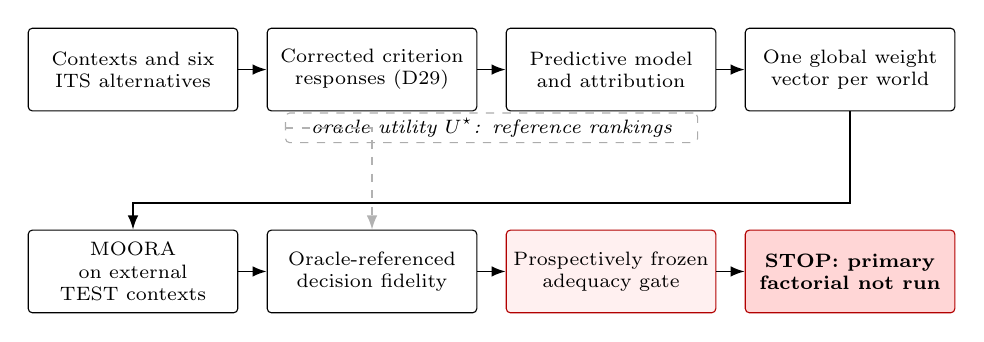
\begin{tikzpicture}[
  node distance=3.2mm and 3.6mm,
  box/.style={draw, rounded corners=1.5pt, align=center, minimum height=10.5mm,
              text width=.205\linewidth, inner sep=2.5pt, font=\scriptsize},
  gate/.style={draw=red!70!black, fill=red!6, rounded corners=1.5pt, align=center,
               minimum height=10.5mm, text width=.205\linewidth, inner sep=2.5pt,
               font=\scriptsize},
  stop/.style={draw=red!70!black, fill=red!16, rounded corners=1.5pt, align=center,
               minimum height=10.5mm, text width=.205\linewidth, inner sep=2.5pt,
               font=\scriptsize\bfseries},
  oracle/.style={draw=gray!65, dashed, rounded corners=1.5pt, align=center,
                 text width=.42\linewidth, inner sep=2pt, font=\scriptsize\itshape},
  arr/.style={-{Latex[length=1.8mm]}, semithick}
]
\node[box] (ctx)  {Contexts and six\\ITS alternatives};
\node[box, right=of ctx]  (resp) {Corrected criterion\\responses (D29)};
\node[box, right=of resp] (attr) {Predictive model\\and attribution};
\node[box, right=of attr] (wts)  {One global weight\\vector per world};

\node[box, below=15mm of ctx]  (moora) {\MOORA{} on external\\TEST contexts};
\node[box, right=of moora] (fid)   {Oracle-referenced\\decision fidelity};
\node[gate, right=of fid]  (gatee) {Prospectively frozen\\adequacy gate};
\node[stop, right=of gatee] (stopn) {STOP: primary\\factorial not run};

\draw[arr] (ctx)  -- (resp);
\draw[arr] (resp) -- (attr);
\draw[arr] (attr) -- (wts);
\draw[arr] (wts.south) -- ++(0,-11.6mm) -| ([xshift=0mm]moora.north);
\draw[arr] (moora) -- (fid);
\draw[arr] (fid)   -- (gatee);
\draw[arr] (gatee) -- (stopn);
% The oracle runs alongside the learned pipeline and supplies the reference
% rankings that decision fidelity is scored against.
\node[oracle] (orc) at ($(resp)!0.5!(attr) + (0,-7.4mm)$)
  {oracle utility $U^\star$: reference rankings};
\draw[arr,dashed,gray!60] (orc.west) -| (fid.north);
\end{tikzpicture}
\caption{Study logic. Estimation partitions (FIT and WEIGHT) support model fitting and
global-weight estimation; disjoint external TEST contexts support \MOORA{} decisions
and oracle-referenced fidelity. The gate decides whether the protected primary
comparison is scientifically warranted; here it decided against.}
\label{fig:workflow}
\end{figure}

% ============================================================
\section{Related Work and Contribution Boundary}
\label{sec:related}
% ============================================================

XAI--MCDM studies have shown that model explanations can be integrated with ranking
methods across domains including transport and infrastructure
\cite{ciano2025xaimcdm,demir2025shapmultimoora,zakeri2024mlmcdm}, while objective
weighting methods such as \CRITIC{} and entropy derive weights from dispersion and
conflict within a decision matrix
\cite{diakoulaki1995critic,shannon1948,mukhametzyanov2021objective}. These families
answer different questions: attribution summarizes a predictive functional, regression
and permutation summarize supervised association, and objective weights summarize the
observed criterion matrix. Their outputs are numerically comparable but are not
interchangeable notions of preference.

Synthetic XAI benchmarks typically compare explanations against known attribution
targets \cite{liu2021xaibench,agarwal2022openxai}. Our focus lies one step downstream.
Even exact recovery of a global attribution functional need not recover
context-specific oracle choices once that functional has been compressed into a single
fixed weight vector and passed through an aggregation rule. Prediction, attribution and
decision fidelity can fail at different stages, so we evaluate learned SHAP alongside a
matched closed-form oracle attribution using ranking, Top-1 and regret metrics.

The contribution boundary is deliberately narrow. This study does not estimate
empirical ITS effects, does not elicit stakeholder preferences, does not identify a
preferred real-world intervention, and does not test whether SHAP works in general. ITS
supplies a controlled applied decision setting. The scientific object is the adequacy
of a global-weight XAI--MCDM benchmark at one prospectively specified development
reference condition.

% ============================================================
\section{Benchmark and Validation Design}
\label{sec:methods}
% ============================================================

\subsection{An ITS Decision Laboratory}
\label{sec:lab}

The benchmark compares six deployment packages at a common first-stage prioritisation
level (Table~\ref{tab:alternatives}). They represent deployable ITS and
transport-systems-management families rather than city-specific calibrated effects
\cite{fhwa2016corridors,fhwa2017atm,usdotv2x}.

\begin{table}[t]
\centering
\caption{ITS alternatives in the controlled decision laboratory.}
\label{tab:alternatives}
\small
\begin{tabularx}{\linewidth}{@{}c l X@{}}
\toprule
\textbf{ID} & \textbf{Alternative} & \textbf{Operational scope}\\
\midrule
$A_1$ & ATSC & Adaptive phase, split, offset or cycle decisions.\\
$A_2$ & TSP & Transit-priority requests and signal responses.\\
$A_3$ & TIDM & Incident detection, verification, response and recovery.\\
$A_4$ & RMTI--DRG & Real-time multimodal information and dynamic route guidance.\\
$A_5$ & V2X--CS & Cooperative safety warnings, excluding signal timing and TSP.\\
$A_6$ & DSM & Dynamic speed management and harmonisation.\\
\bottomrule
\end{tabularx}
\end{table}

Ten benefit-oriented criteria cover mobility efficiency, reliability,
person-throughput, safety, resilience, environmental efficiency, accessibility,
readiness, interoperability/scalability and direction-adjusted lifecycle burden, driven
by five correlated latent factors: demand, incidents, person movement, environmental
sensitivity and infrastructure readiness.

\emph{Each replication seed defines one benchmark world}: its technology parameters,
its contexts and all of its random streams. The world is the statistical unit
throughout this paper. Alternative--context rows are never treated as independent
population replications.

\subsection{A Structural Defect and the D29 Correction}
\label{sec:generator}

The initial noise-free response for the seven active criteria $C_1$--$C_7$ had the form
\begin{equation}
g_{asj}=\theta_{aj}\,o_{sj},
\label{eq:separable}
\end{equation}
where $a$, $s$ and $j$ index alternative, context and criterion, $\theta_{aj}$ is a
capability amplitude and $o_{sj}$ a context opportunity. Under the vector
normalization used by the decision operator, for $o_{sj}>0$,
\begin{equation}
r_{asj}
=\frac{\theta_{aj}o_{sj}}{\sqrt{\sum_b\theta_{bj}^2o_{sj}^2}}
=\frac{\theta_{aj}}{\sqrt{\sum_b\theta_{bj}^2}}.
\label{eq:collapse}
\end{equation}
The common opportunity term cancels exactly, so every context yields an identical
normalized column. Sum, max and min--max normalizations exhibit the same common-scale
cancellation. This answers RQ1: raw contextual variation, on its own, was not evidence
that the benchmark posed a context-sensitive decision problem, and only a diagnostic
applied \emph{at the operator's normalization} could reveal it.

After prospectively separated calibration and eligibility screening, the frozen
correction---referred to as the D29 kernel---for the active $C_1$--$C_7$ pathways was
\begin{equation}
g_{asj}=\theta_{aj}o_{sj}+0.05\,v_{aj}\,o_{sj}(1-o_{sj}),
\qquad v_{aj}\in[-1,1].
\label{eq:d29}
\end{equation}
The deterministic contrast values $v_{aj}$ were assigned without any outcome or winner
information. Because active $\theta_{aj}\ge0.05$, the response stays monotone on
$o\in[0,1]$. D29 was retained for protocol continuity and minimal intervention among
$54$ corrected-eligible candidates, not because it produced a preferred ITS winner or a
favourable method comparison. The rejected families and the full candidate history are
supplementary.

\subsection{Oracle, Global Weights and the Decision Operator}
\label{sec:oracle}

Benefit-oriented criterion values are passed through $q_j(g)=\log(1+2g)/\log 3$. The
noise-free oracle utility is
\begin{equation}
U_{as}^{\star}
=\frac{\sum_{j=1}^{10}\alpha_j q_j(g_{asj})
+\lambda\sum_{(j,k)\in\mathcal E}0.20\,q_j(g_{asj})q_k(g_{ask})}
{1+\lambda}.
\label{eq:oracle}
\end{equation}
This is an internally specified reference, not causal truth and not social welfare.
The prediction target adds controlled noise to $U^\star$. Because
Eq.~\eqref{eq:oracle} contains only main effects and pairwise interactions, the frozen
interventional Shapley functional admits a closed-form \emph{oracle attribution}.
Global oracle weights normalize mean absolute WEIGHT-set attributions; learned SHAP
applies the same aggregation to interventional TreeSHAP values from a fixed \XGB{}
model \cite{chen2016xgboost,lundberg2020trees}.

Six structured global-weight methods enter the gate: oracle attribution, SHAP,
fixed-model context-block permutation importance (PI), non-negative Ridge+, \CRITIC{}
and entropy. Equal, RandomWeights and MajorityWinner serve as diagnostic references.
Every weighting method produces exactly one context-invariant vector per world, which
is the point: the design deliberately asks what survives that compression. Estimation
uses disjoint FIT and WEIGHT partitions, and the $200$ external TEST contexts are never
used for fitting or weight estimation. At the Pilot-B size $N=250$, each world holds
$200$ FIT, $50$ WEIGHT and $200$ TEST contexts.

The downstream operator is benefit-oriented weighted \MOORA{} \cite{brauers2006moora}:
\begin{equation}
r_{asj}=\frac{g_{asj}}{\sqrt{\sum_{b=1}^{6}g_{bsj}^2}+10^{-12}},
\qquad
S_{as}=\sum_{j=1}^{10}w_j r_{asj}.
\label{eq:moora}
\end{equation}
Alternatives are ranked by descending $S_{as}$. All score representations use an
absolute $10^{-12}$ tie tolerance, anchor-based average ranks without tie chaining, and
ascending alternative ID for deterministic Top-1 selection.

\subsection{Decision Fidelity and the Prospective Adequacy Gate}
\label{sec:gate}

Agreement with the oracle is measured three ways: full-ranking agreement by Kendall's
$\tau_b$, deterministic Top-1 accuracy, and normalized oracle regret
\begin{equation}
R_s^{(q)}=
\frac{U_{a_s^\star,s}^{\star}-U_{\hat a_s^{(q)},s}^{\star}}
{\max_a U_{as}^{\star}-\min_a U_{as}^{\star}+10^{-12}}.
\label{eq:regret}
\end{equation}

Pilot B was frozen before execution at $(N,c,\rho,\lambda)=(250,0.30,0.4,0.5)$ over
development worlds 21001--21005. It uses $200$ common
$\operatorname{Dirichlet}(1,\ldots,1)$ RandomWeights draws per world and one
MajorityWinner per world.

MajorityWinner is an oracle-informed diagnostic reference. It is the context-free
oracle-modal alternative estimated on WEIGHT and evaluated on TEST---the constant
alternative maximizing empirical oracle Top-1 frequency on WEIGHT. It is not claimed to
minimize regret or to constitute an operational transportation policy, and it is
neither stakeholder-derived nor normative. It is included precisely because it is
strong and cheap: a global-weight pipeline should add decision value beyond a single
constant choice before its additional complexity is considered justified.

A practical method advantage must be strictly positive in at least four of the five
worlds \emph{and} meet the relevant cross-world median margin.
Table~\ref{tab:gates} lists the five independently sufficient stop conditions. The
overall rule is an OR: the benchmark passes only if every stop is false. The margins
are design-specific adequacy tolerances, not universal equivalence bounds.

\begin{table}[t]
\centering
\caption{The five prospectively frozen Pilot-B stop conditions. Any one of them halts
the study; passage requires all five to be false.}
\label{tab:gates}
\small
\begin{tabularx}{\linewidth}{@{}l X@{}}
\toprule
\textbf{Stop} & \textbf{Condition}\\
\midrule
Coverage & A required structured output or RandomWeights coverage is missing.\\
Random equivalence & No method clears median $\Delta\tau_b=0.05$ or
$\Delta$mean-regret $=0.01$ versus RandomWeights.\\
Modal-winner tie & No method clears median $\Delta$Top-1 $=0.02$ or
$\Delta$mean-regret $=0.01$ versus MajorityWinner.\\
Oracle dominance & Pooled oracle modal share is at least $0.90$.\\
Weight insensitivity & Random-weight choices or performance widths meet the frozen
invariance criteria.\\
\bottomrule
\end{tabularx}
\end{table}

The protocol, the evaluator and the protected-seed firewall were committed before the
single authorized execution. A 30-world, 135-cell primary factorial and its associated
robustness analyses were conditional on Pilot-B passage. They were not run. This is
version-controlled prospective specification rather than public preregistration; the
complete provenance appears in the supplement.

% ============================================================
\section{Results}
\label{sec:results}
% ============================================================

\subsection{Structural Validity Did Not Guarantee Decision Diversity}
\label{sec:structural}

The historical generator of Eq.~\eqref{eq:separable} collapsed numerically exactly
where the algebra predicted. Across all $35$ world--criterion combinations the maximum
active-pair log-ratio variation was $7.2224\times10^{-16}$ and the maximum
vector-normalized profile variation was $1.8036\times10^{-9}$: machine noise, not
signal.

The corrected D29 kernel cleared the frozen structural and reachability requirements,
and it did produce multiple oracle orderings and multiple oracle winners in every
world---between $17$ and $78$ distinct complete orderings and between two and five
distinct winners. Yet its oracle decision geometry stayed markedly uneven. The modal
oracle winner's share ranged from $0.519$ to $0.983$ across the five worlds, with a
median of $0.809$. In world 21001, the directly comparable case, the correction raised
the number of distinct oracle orderings from $19$ to $23$ while also raising modal
share from $0.962$ to $0.983$.

Removing exact multiplicative separability was therefore necessary for this benchmark
but not sufficient. In three of five worlds a single alternative was already
oracle-optimal in over $80\%$ of contexts, which sets a high bar for any pipeline that
must beat a constant choice.

\subsection{The Pilot-B Result}
\label{sec:pilotb}

All six structured methods were defined in every world, every required Kendall summary
was available, and no Equal fallback was used. Table~\ref{tab:gateoutcome} reports the
independently reconstructed gate decision. Four of six methods separated from
RandomWeights, so the random-equivalence stop was false. The pooled oracle modal share
was $0.526$ ($A_2$ in $526$ of $1000$ TEST contexts), so no single alternative
dominated the pooled worlds, and RandomWeights decisions were not invariant. Exactly
one stop fired: the modal-winner effective tie.

\begin{table}[t]
\centering
\caption{Frozen Pilot-B outcome. The overall hard stop is the OR of the five flags;
one flag fired.}
\label{tab:gateoutcome}
\small
\begin{tabularx}{\linewidth}{@{}lXc@{}}
\toprule
Gate & Audited result & Stop\\
\midrule
Coverage & Six structured methods eligible without fallback & No\\
Random equivalence & Four of six methods separated from RandomWeights & No\\
Modal-winner tie & Zero of six methods escaped MajorityWinner & \textbf{Yes}\\
Oracle dominance & Pooled modal share $0.526<0.90$ & No\\
Weight insensitivity & Invariant fraction $0.004<0.90$; qualified worlds $0<4$ & No\\
\midrule
Overall & At least one prospectively frozen stop fired & \textbf{Yes}\\
\bottomrule
\end{tabularx}
\end{table}

Table~\ref{tab:contrasts} and Fig.~\ref{fig:contrast} localize the failure; positive
values favour the structured method. Oracle attribution, SHAP, PI and Ridge+ each
cleared a RandomWeights criterion with the required cross-world consistency. SHAP
showed the largest median Kendall improvement, $0.288$, positive in all five worlds,
together with a median regret improvement of $0.026060$, positive in four. Against
MajorityWinner, by contrast, SHAP's median Top-1 and median regret advantages were both
exactly zero, with only two positive worlds. No method met either modal-winner margin
with the required four-of-five consistency.

The compact statement of the whole result is this. \emph{Four structured methods,
including SHAP, cleared the prospectively specified RandomWeights adequacy criterion,
but no structured method cleared the prospectively specified MajorityWinner adequacy
criterion.}

\begin{table}[t]
\centering
\caption{Cross-world median Pilot-B contrasts, with the count of strictly positive
worlds in parentheses (P, out of five). MW denotes MajorityWinner, RW RandomWeights.
The last column reports the frozen RandomWeights separation verdict.}
\label{tab:contrasts}
\scriptsize
\setlength{\tabcolsep}{2.5pt}
\begin{tabular}{@{}lrrrrc@{}}
\toprule
Method & \shortstack{MW\\$\Delta$Top-1 (P)} & \shortstack{MW\\$\Delta$regret (P)} &
\shortstack{RW\\$\Delta\tau_b$ (P)} & \shortstack{RW\\$\Delta$regret (P)} & RW sep.\\
\midrule
Oracle attribution & $-0.010$ (1) & $-0.002119$ (1) & $0.209$ (5) & $0.023940$ (4) & Yes\\
SHAP & $0.000$ (2) & $0.000000$ (2) & $0.288$ (5) & $0.026060$ (4) & Yes\\
Permutation importance & $-0.120$ (1) & $-0.004425$ (1) & $0.194$ (5) & $0.010658$ (4) & Yes\\
Ridge+ & $-0.010$ (1) & $-0.002119$ (1) & $0.237$ (5) & $0.011492$ (4) & Yes\\
CRITIC & $-0.580$ (0) & $-0.124414$ (0) & $0.030$ (3) & $-0.098354$ (0) & No\\
Entropy & $-0.580$ (0) & $-0.156641$ (0) & $0.035$ (3) & $-0.002807$ (1) & No\\
\bottomrule
\end{tabular}
\end{table}

\begin{figure}[t]
\centering
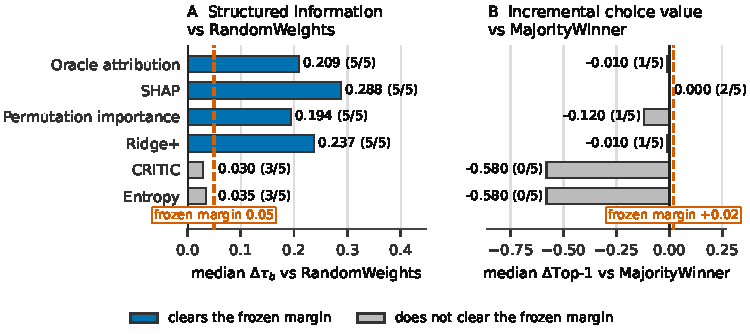
\includegraphics[width=\linewidth]{decision_value_figure}
\caption{Information learned is not decision value added. Left: every structured
method except \CRITIC{} and entropy clears the frozen $0.05$ Kendall margin against
RandomWeights. Right: no method reaches the frozen $+0.02$ Top-1 margin against the
constant MajorityWinner reference, and SHAP's advantage there is exactly zero. Both
panels are drawn directly from the frozen Pilot-B result on a common untruncated
scale.}
\label{fig:contrast}
\end{figure}

The exact oracle-attribution reference failed the same gate, so the stop cannot be
attributed to \XGB{} fitting error or TreeSHAP approximation alone.

\subsection{Post-Closure Descriptive Selection Maps}
\label{sec:selectionmaps}

The Pilot-B artefact retained aggregate metrics but not method-level context
selections. After permanent closure, a separate protocol was frozen before any
selection was reconstructed. It reused the archived fixed weights and TEST identities,
generated no target, fitted or queried no model, re-estimated no weight, and could not
alter the gate; an independent audit verified all $5\times7\times200=7000$ selections.
This is a post-closure descriptive diagnostic and has no confirmatory role.

Equal-weight \MOORA{} selected a single alternative in every context of every world and
matched MajorityWinner exactly in four of five worlds. Structured-method constancy was
heterogeneous, from zero worlds for PI to three for entropy
(Table~\ref{tab:selectionmaps}). The simple hypothesis that every fixed-weight \MOORA{}
vector must be context invariant is therefore not supported for the seven observed
vectors. World 21003 also shows why Top-1 and full-ranking fidelity must be reported
separately: Equal, \CRITIC{} and entropy all selected $A_6$ in all $200$ contexts,
giving identical Top-1 accuracy $0.190$ and mean regret $0.316758$, while their mean
$\tau_b$ values still differed ($0.5493$, $0.5427$, $0.5113$) because the lower ranks
differed. These observations suggest locally coarse decision regions for particular
fixed vectors. They do not characterize unobserved weight space, do not establish a
causal mechanism for the Pilot-B stop, and do not change its outcome.

\begin{table}[t]
\centering
\caption{Post-closure descriptive diagnostic over the seven observed fixed vectors.
Counts give worlds with a single selected alternative, and worlds with exact
context-level agreement with MajorityWinner. Descriptive only; non-confirmatory.}
\label{tab:selectionmaps}
\small
\begin{tabular}{@{}l@{\hspace{2em}}c@{\hspace{2em}}c@{}}
\toprule
Method & Constant-selection worlds & All-context MW-match worlds\\
\midrule
Oracle attribution & 1/5 & 1/5\\
SHAP & 2/5 & 2/5\\
Permutation importance & 0/5 & 0/5\\
Ridge+ & 1/5 & 1/5\\
CRITIC & 2/5 & 1/5\\
Entropy & 3/5 & 2/5\\
Equal & 5/5 & 4/5\\
\bottomrule
\end{tabular}
\end{table}

% ============================================================
\section{Discussion}
\label{sec:discussion}
% ============================================================

\subsection{What the Study Establishes}
\label{sec:establishes}

RQ1 and RQ2 are addressed by the prospectively structured benchmark-development and
Pilot-B evidence. The separately frozen post-closure diagnostic addresses DQ1
descriptively and has no confirmatory role.

For RQ1, an algebraic and numerical audit showed that contextual variation can vanish
entirely under the normalization used by the decision operator, and that a diagnostic
must be applied at that point to detect it. For RQ2, correcting exact separability
produced multiple oracle orderings and winners in every world, but it did not establish
sufficient incremental decision value: no structured global-weight pipeline escaped
MajorityWinner under the frozen cross-world rule.

The clearest reading is not that SHAP failed. Its separation from RandomWeights shows
that its weights carried reproducible ranking information, and that entire median
advantage then disappeared against a single constant choice: at this reference
condition the bottleneck lay in converting one global weight vector into
context-specific decision value through \MOORA{}. Because closed-form oracle
attribution reached the same outcome, an explanation resting solely on imperfect
learned attribution is ruled out. No single causal mechanism is isolated, however:
generator geometry, global compression, reference construction and \MOORA{} geometry
remain coupled in the executed design.

For applied OR and transport research the lesson is compact. A complex data-driven
pipeline should be compared not only against random or uniform parameters but also
against a meaningful simple decision policy: beating random weights shows that
information was learned, not that it usefully changes the operational choice.

\subsection{Interpretation Boundary and Limitations}
\label{sec:limits}

The central boundary statement is this. \emph{Pilot-B failure denotes failure of the
prespecified adequacy requirement for the intended global-weight--\MOORA{} comparison;
it does not imply that the generator contains no discriminative decision information.}
Four independent observations support the distinction: RandomWeights decisions were not
invariant; four structured methods separated from RandomWeights; SHAP held a large and
consistent Kendall advantage; and the observed fixed vectors displayed heterogeneous
selection constancy rather than uniform collapse. Equally, the result does not show
that SHAP universally fails, that global weights never matter, that \MOORA{} is
generally inadequate, that the D29 kernel is defective, that one ITS alternative is
best, or that MajorityWinner should be deployed.

Ten limitations bound the claim.

\begin{enumerate}
\itemsep1pt
\item Pilot B uses only five worlds, so cross-world inferential precision is low.
\item Those five are reused development worlds, not fresh ones.
\item Only one reference condition was evaluated, $(N,c,\rho,\lambda)=(250,0.30,0.4,0.5)$.
\item \emph{Prospective freezing prevents post-result modification of the gate, but it
does not make the five reused development worlds independent validation data.} The
result is a protocol-level adequacy screen; no population-level inference about method
performance is claimed.
\item MajorityWinner headroom varies strongly across worlds, from a modal share of
$0.519$ to $0.983$, so the difficulty of the comparison is itself heterogeneous.
\item MajorityWinner is Top-1-derived, not regret-optimal. The regret arm uses the same
prospectively frozen Top-1-derived constant reference rather than a separately
optimized regret-minimizing constant policy. A future benchmark could prospectively
define metric-matched constant references.
\item The generator, oracle and capability mask are synthetic assumptions, not
empirical transport effects, causal truth, stakeholder preferences or social welfare.
\item Every global-weight method intentionally compresses context-specific information,
and the methods differ in semantics: oracle attribution and SHAP target one
interventional functional; Ridge+ and PI use supervised association; \CRITIC{} and
entropy summarize pooled decision-matrix properties. PI can additionally extrapolate
when dependence is broken \cite{hooker2021permutation}.
\item The post-closure diagnostic adds no independent worlds. A paired context
bootstrap was prospectively excluded from that layer and was not executed; any
resampling study would require its own protocol and could not reopen the gate.
\item The paper makes no empirical ITS deployment recommendation.
\end{enumerate}

The negative result stays scientifically useful because it was not tuned away. The
generator correction, the gate thresholds, the evaluator and the seed firewall all
preceded the authorized result. Once the modal-winner stop fired, the 30-world primary
factorial and the reserve worlds remained barred. Any future design must begin as a
separately versioned study that discloses this closed result rather than retroactively
amending it.

% ============================================================
\section{Conclusion}
\label{sec:conclusion}
% ============================================================

This study asked whether a synthetic ITS benchmark could support a global XAI--MCDM
method comparison, and it asked before running the comparison at scale. Structural
auditing found and corrected a normalization-induced collapse in the original
generator, but that correction, while necessary, did not by itself establish downstream
decision discrimination. At the frozen development reference, four structured
methods---SHAP among them---cleared the RandomWeights adequacy criterion, yet none
cleared the MajorityWinner criterion, and closed-form oracle attribution failed the
same gate.

The defensible conclusion is narrow and actionable: at this reference condition the
evaluated global-weight-compression--\MOORA{} pipelines did not establish enough
incremental decision value to justify the protected primary factorial, and the gate
therefore performed its intended function. More broadly, synthetic XAI--MCDM studies
should validate not only prediction and attribution, but also whether the benchmark can
discriminate decisions beyond meaningful simple references. In XAI-assisted decision
support, recovering structured importance is not enough; the recovered information must
demonstrably change decisions in a useful way.

% ============================================================
\section*{Code and Data Availability}

The reproducibility package contains the synthetic benchmark generator, the frozen
configuration and protocol files, the deterministic seed definitions, the archived
development-audit and Pilot-B result artefacts, the frozen global-weight vectors, the
post-closure selection-map outputs, the independent audit and evaluator scripts, the
software-environment specification, content-integrity manifests, and the read-only
scripts that regenerate every table and figure reported here. Raw benchmark worlds are
regenerated deterministically from the frozen seeds and configurations rather than
stored as large duplicated datasets. Primary and reserve worlds were never accessed and
no primary result exists.
\ifanon
During double-blind review, identifying repository metadata is withheld; an anonymous
archive can be supplied to editors and reviewers on request. The complete
version-controlled repository and its immutable provenance record will be released
publicly after review.
\else
The complete version-controlled repository and its immutable provenance record are
released with the public reproducibility package.
\fi

\ifanon
\else
\section*{CRediT Authorship Contribution Statement}

\textbf{Mohamed Yassine Neifar:} Conceptualization, Methodology, Software, Validation,
Formal analysis, Investigation, Data curation, Visualization, Writing -- original
draft, Writing -- review and editing.
\textbf{Nadir Farhi:} Conceptualization, Methodology, Validation, Supervision,
Writing -- review and editing.
\textbf{Ahmed Frikha:} Supervision, Writing -- review and editing.
\fi

\section*{Funding}

This research did not receive any specific grant from funding agencies in the public,
commercial, or not-for-profit sectors.

\section*{Declaration of Competing Interest}

The authors declare that they have no known competing financial interests or personal
relationships that could have appeared to influence the work reported in this paper.

\section*{Declaration of Generative AI and AI-Assisted Technologies}

Generative AI tools were used for language editing, manuscript organization,
consistency checking and LaTeX assistance. All scientific design decisions, code
executions, numerical results, interpretations and citations were independently checked
by the authors, who take full responsibility for the manuscript.

\ifanon
\else
\section*{Acknowledgements}

The authors acknowledge the academic guidance and scientific support provided within
the doctoral research collaboration between the University of Sfax and Universit\'e
Gustave Eiffel.
\fi

% ============================================================
\begin{thebibliography}{99}

\bibitem{keeney1976decisions}
Keeney, R.L., Raiffa, H.:
Decisions with Multiple Objectives: Preferences and Value Tradeoffs.
Wiley, New York (1976).

\bibitem{roy1996importance}
Roy, B., Mousseau, V.:
A theoretical framework for analysing the notion of relative importance of criteria.
Journal of Multi-Criteria Decision Analysis \textbf{5}(2), 145--159 (1996).
\url{https://doi.org/10.1002/(SICI)1099-1360(199606)5:2<145::AID-MCDA99>3.0.CO;2-5}

\bibitem{choo1999weights}
Choo, E.U., Schoner, B., Wedley, W.C.:
Interpretation of criteria weights in multicriteria decision making.
Computers \& Industrial Engineering \textbf{37}(3), 527--541 (1999).
\url{https://doi.org/10.1016/S0360-8352(00)00019-X}

\bibitem{mukhametzyanov2021objective}
Mukhametzyanov, I.:
Specific character of objective methods for determining weights of criteria in MCDM
problems: Entropy, CRITIC and SD.
Decision Making: Applications in Management and Engineering \textbf{4}(2), 76--105
(2021).
\url{https://doi.org/10.31181/dmame210402076i}

\bibitem{chen2016xgboost}
Chen, T., Guestrin, C.:
XGBoost: A scalable tree boosting system.
In: Proceedings of the 22nd ACM SIGKDD International Conference on Knowledge Discovery
and Data Mining, pp. 785--794 (2016).
\url{https://doi.org/10.1145/2939672.2939785}

\bibitem{lundberg2017shap}
Lundberg, S.M., Lee, S.-I.:
A unified approach to interpreting model predictions.
In: Advances in Neural Information Processing Systems, vol. 30 (2017).

\bibitem{lundberg2020trees}
Lundberg, S.M., Erion, G., Chen, H., et al.:
From local explanations to global understanding with explainable AI for trees.
Nature Machine Intelligence \textbf{2}, 56--67 (2020).
\url{https://doi.org/10.1038/s42256-019-0138-9}

\bibitem{sundararajan2020many}
Sundararajan, M., Najmi, A.:
The many Shapley values for model explanation.
In: Proceedings of the 37th International Conference on Machine Learning,
PMLR \textbf{119}, 9269--9278 (2020).

\bibitem{kumar2020shapleyproblems}
Kumar, I.E., Venkatasubramanian, S., Scheidegger, C., Friedler, S.:
Problems with Shapley-value-based explanations as feature importance measures.
In: Proceedings of the 37th International Conference on Machine Learning,
PMLR \textbf{119}, 5491--5500 (2020).

\bibitem{janzing2020causal}
Janzing, D., Minorics, L., Bl{\"o}baum, P.:
Feature relevance quantification in explainable AI: A causal problem.
In: Proceedings of the 23rd International Conference on Artificial Intelligence and
Statistics, PMLR \textbf{108}, 2907--2916 (2020).

\bibitem{hooker2021permutation}
Hooker, G., Mentch, L., Zhou, S.:
Unrestricted permutation forces extrapolation: Variable importance requires at least
one more model, or there is no free variable importance.
Statistics and Computing \textbf{31}, 82 (2021).
\url{https://doi.org/10.1007/s11222-021-10057-z}

\bibitem{liu2021xaibench}
Liu, Y., Khandagale, S., White, C., Neiswanger, W.:
Synthetic benchmarks for scientific research in explainable machine learning.
Proceedings of the Neural Information Processing Systems Track on Datasets and
Benchmarks \textbf{1} (2021).

\bibitem{agarwal2022openxai}
Agarwal, C., Krishna, S., Saxena, E., Pawelczyk, M., Johnson, N., Puri, I., Zitnik, M.,
Lakkaraju, H.:
OpenXAI: Towards a transparent evaluation of model explanations.
In: Advances in Neural Information Processing Systems, vol. 35, Datasets and Benchmarks
Track (2022).

\bibitem{ciano2025xaimcdm}
Ciano, T., Ferrara, M.:
Explainable multi-criteria decision making for tourism economics: Integrating XAI with
MCDM for a robust accommodation performance assessment.
Decisions in Economics and Finance (2025).
\url{https://doi.org/10.1007/s10203-025-00553-6}

\bibitem{demir2025shapmultimoora}
Demir, A.S., Da{\u g}deviren, U., Kurnaz, T.F., Erden, C., K{\"o}k{\c c}am, A.H.:
An integrated SHAP-MCDM approach for slope stability prediction based on machine
learning algorithms.
Natural Hazards \textbf{121}(18), 21811--21836 (2025).
\url{https://doi.org/10.1007/s11069-025-07665-7}

\bibitem{zakeri2024mlmcdm}
Zakeri, S., Konstantas, D., Sorooshian, S., Chatterjee, P.:
A novel ML-MCDM-based decision support system for evaluating autonomous vehicle
integration scenarios in Geneva's public transportation.
Artificial Intelligence Review \textbf{57}, 310 (2024).
\url{https://doi.org/10.1007/s10462-024-10917-w}

\bibitem{diakoulaki1995critic}
Diakoulaki, D., Mavrotas, G., Papayannakis, L.:
Determining objective weights in multiple criteria problems: The CRITIC method.
Computers \& Operations Research \textbf{22}(7), 763--770 (1995).
\url{https://doi.org/10.1016/0305-0548(94)00059-H}

\bibitem{shannon1948}
Shannon, C.E.:
A mathematical theory of communication.
Bell System Technical Journal \textbf{27}, 379--423, 623--656 (1948).

\bibitem{brauers2006moora}
Brauers, W.K.M., Zavadskas, E.K.:
The MOORA method and its application to privatization in a transition economy.
Control and Cybernetics \textbf{35}(2), 445--469 (2006).

\bibitem{fhwa2016corridors}
Federal Highway Administration:
Planning for Transportation Systems Management and Operations Within Corridors: A Desk
Reference, FHWA-HOP-16-037 (2016).
\url{https://ops.fhwa.dot.gov/Publications/fhwahop16037/}

\bibitem{fhwa2017atm}
Kuhn, B., Balke, K., Wood, N.:
Active Traffic Management (ATM) Implementation and Operations Guide.
FHWA-HOP-17-056, Federal Highway Administration (2017).
\url{https://ops.fhwa.dot.gov/publications/fhwahop17056/}

\bibitem{usdotv2x}
U.S. Department of Transportation, ITS Joint Program Office:
V2X Applications and Use Cases.
\url{https://its.dot.gov/research-areas/V2X-Deployment/overview/v2x-applications/}
(accessed 13 August 2026).

\bibitem{morris2019simulation}
Morris, T.P., White, I.R., Crowther, M.J.:
Using simulation studies to evaluate statistical methods.
Statistics in Medicine \textbf{38}(11), 2074--2102 (2019).
\url{https://doi.org/10.1002/sim.8086}

\bibitem{niessl2022overoptimism}
Nie{\ss}l, C., Herrmann, M., Wiedemann, C., Casalicchio, G., Boulesteix, A.-L.:
Over-optimism in benchmark studies and the multiplicity of design and analysis options
when interpreting their results.
WIREs Data Mining and Knowledge Discovery \textbf{12}(2), e1441 (2022).
\url{https://doi.org/10.1002/widm.1441}

\end{thebibliography}

\end{document}
"
%
% No numerical result in this file may be edited by hand. Every reported value
% is verified against the frozen artefacts by
%   scripts/paper/verify_frozen_manuscript_numbers.py
% ============================================================
% ChkTeX: intentional en dashes, citation spacing, label placement, acronym
% punctuation and LNCS bibliography conventions.
% chktex-file 2
% chktex-file 8
% chktex-file 13
% chktex-file 24
% chktex-file 36

\documentclass[runningheads,orivec]{llncs}

\usepackage[T1]{fontenc}
\usepackage[utf8]{inputenc}
\usepackage{amsmath,amssymb,amsfonts}
\usepackage{booktabs}
\usepackage{tabularx}
\usepackage{graphicx}
\usepackage{tikz}
\usetikzlibrary{arrows.meta,positioning,calc}
\usepackage{hyperref}

\hypersetup{hidelinks}
\graphicspath{{../outputs/paper/figures/}{./figures/}{./}}

% ---- build-mode switch: anonymous by default -----------------
\providecommand{\CAMERAREADY}{0}
\newif\ifanon
\anontrue
\ifnum\CAMERAREADY=1 \anonfalse \fi
% --------------------------------------------------------------

\newcommand{\XGB}{XGBoost}
\newcommand{\MOORA}{MOORA}
\newcommand{\CRITIC}{CRITIC}
\newcommand{\E}{\mathbb{E}}

\begin{document}
\emergencystretch=1.5em

\title{From Predictive Importance to Decision Value: Evaluating XAI-Based
Weights for ITS Prioritisation}
\titlerunning{From Predictive Importance to Decision Value}

\ifanon
  \author{Anonymous Author(s)}
  \authorrunning{Anonymous Author(s)}
  \institute{Anonymous Institution(s)}
\else
  \author{Mohamed Yassine Neifar\inst{1,2}\thanks{Corresponding author.} \and
  Ahmed Frikha\inst{2} \and
  Nadir Farhi\inst{1}}
  \authorrunning{Neifar et al.}
  \institute{Universit\'e Gustave Eiffel, COSYS--GRETTIA,
  14--20 Boulevard Newton, Cit\'e Descartes, Champs-sur-Marne,
  F-77447 Marne-la-Vall\'ee Cedex 2, France
  \and
  Institut Sup\'erieur de Gestion Industrielle de Sfax (ISGIS),
  OLID, University of Sfax, Route de l'A\'eroport km 4, BP 1099,
  Sfax 3038, Tunisia\\
  \email{yessine.neifar.imsil@isgis.usf.tn}}
\fi

\maketitle

\begin{abstract}
Feature attributions from predictive models are increasingly rescaled into global
criterion weights for multi-criteria decision-making. Predictive importance and
decision value are, however, different quantities, and a benchmark must be able to
tell them apart before it can compare methods. We build a controlled synthetic
laboratory for Intelligent Transportation Systems prioritisation: six alternatives,
ten criteria, a nonlinear oracle, \XGB, interventional TreeSHAP, six structured
global-weight pipelines and benefit-oriented \MOORA. A structural audit first showed
that the original generator's apparent contextual variation cancelled exactly under
the normalization used by the decision operator. A corrected monotone response kernel
removed that algebraic collapse. We then executed a five-world adequacy gate that had
been frozen before execution. Four structured methods, including SHAP, cleared the
prospectively specified RandomWeights adequacy criterion; SHAP reached a median
Kendall $\tau_b$ improvement of $0.288$, positive in all five worlds. No structured
method cleared the MajorityWinner criterion---SHAP's median Top-1 and regret
advantages against that constant reference were exactly zero---and closed-form oracle
attribution failed the same gate, so the outcome is not an artefact of learned
approximation. The gate therefore stopped the protected primary factorial. Recovering
structured importance is not sufficient: synthetic XAI--MCDM benchmarks should
demonstrate incremental decision value against meaningful simple references before
comparing methods.

\keywords{Explainable AI \and Multi-Criteria Decision-Making \and Benchmark Validity
\and Prospective Stopping \and Decision Support \and Intelligent Transportation
Systems}
\end{abstract}

% ============================================================
\section{Introduction}
\label{sec:introduction}
% ============================================================

Transport agencies routinely prioritise Intelligent Transportation Systems (ITS) with
limited operational evidence and limited capacity for formal preference elicitation.
The task is naturally multi-criteria: candidate deployments differ in mobility,
reliability, person-throughput, safety, environmental performance, accessibility,
readiness, interoperability and lifecycle burden. Machine learning and explainable
artificial intelligence (XAI) offer an attractive shortcut. Fit a performance model,
aggregate its feature attributions into criterion ``importance'', normalize the result
into weights, and rank alternatives with a multi-criteria decision-making (MCDM) rule.

That shortcut contains a semantic leap and an empirical one. MCDM weights take their
meaning from criterion scales and from the aggregation model; they are not generic
measures of importance \cite{keeney1976decisions,roy1996importance,choo1999weights}.
SHAP values allocate model output under a specified cooperative-game functional
\cite{lundberg2017shap}, but a predictive attribution is not automatically a
stakeholder preference, a causal effect or a valid trade-off constant
\cite{sundararajan2020many,kumar2020shapleyproblems,janzing2020causal}. Consequently
\[
\text{predictive attribution}
\;\longrightarrow\;
\text{global criterion weight}
\;\longrightarrow\;
\text{MCDM ranking}
\]
is a pipeline to be validated, not an identity to be assumed.

Controlled synthetic studies look well suited to that validation, because the
data-generating process and an oracle reference are both known. Yet a synthetic
benchmark can carry a great deal of raw variation and still pose a nearly trivial
decision problem, and a method comparison run on such a benchmark measures
implementation differences rather than decision value. Benchmark studies are also
vulnerable to over-optimism when generators, estimands or analyses are revised after
method performance has been observed
\cite{morris2019simulation,niessl2022overoptimism}.

We therefore separate two notions and use them consistently throughout.
\emph{Validity} refers to the conceptual scientific properties of the benchmark:
whether its responses vary, whether that variation survives normalization, whether the
oracle is well defined. \emph{Adequacy} refers to the operational, prospectively frozen
test used to decide whether a protected primary comparison is warranted at all. A
benchmark can be valid and still be inadequate.

We address two prospective research questions.

\begin{description}
\item[RQ1.] Can structural diagnostics reveal when apparent contextual variation
disappears under the normalization used by the downstream MCDM operator?
\item[RQ2.] After correcting that structural defect, do structured global-weight
pipelines provide sufficient incremental decision value over random-weight and
constant-decision references to justify protected primary evaluation?
\end{description}

After the study was permanently closed we additionally froze one descriptive
diagnostic, reported here under a deliberately separate label.

\begin{description}
\item[DQ1 (post-closure, descriptive).] After Pilot B was permanently closed, what do
the archived context-level selection maps reveal about the observed decision behaviour
of the seven frozen fixed-weight vectors?
\end{description}

DQ1 is post-closure and descriptive. It is non-confirmatory, and it cannot modify,
reinterpret or reopen the Pilot-B gate. It is reported because it is explanatory, not
because it carries evidential weight.

The paper contributes a validation workflow rather than a new weighting algorithm. It
separates raw variation, structural non-separability and downstream decision
discrimination and shows that the first two do not imply the third; it carries a
closed-form oracle attribution alongside learned SHAP, separating estimation error
from losses created by global compression and aggregation; and it demonstrates a
prospectively frozen adequacy gate that stops a planned comparison when its decision
premise fails. To our knowledge this is a rare prospectively gated controlled
evaluation of whether global attribution-derived weights retain downstream decision
value after MCDM aggregation. The generator genealogy, candidate grids, seed
namespaces, software tests, frozen protocols and unexecuted analyses are preserved in
the companion supplement.

Figure~\ref{fig:workflow} gives the study logic end to end. Three features are
central: estimation data and external TEST contexts are disjoint, an oracle reference
runs in parallel with the learned pipeline, and the final gate is evaluated before the
protected experiment is allowed to start.

\begin{figure}[t]
\centering
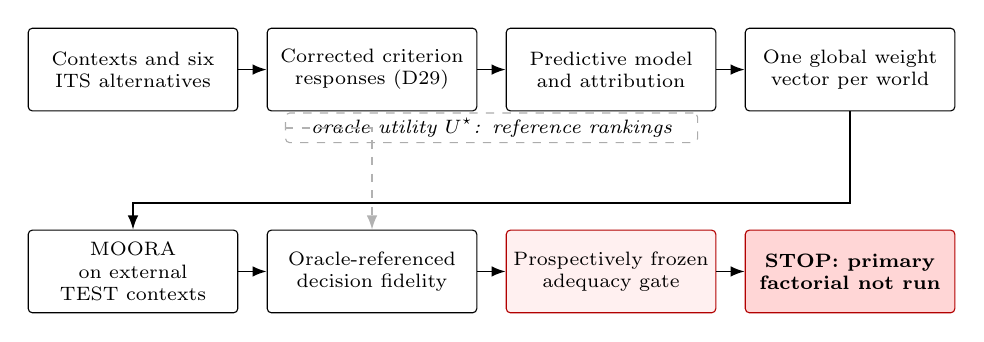
\begin{tikzpicture}[
  node distance=3.2mm and 3.6mm,
  box/.style={draw, rounded corners=1.5pt, align=center, minimum height=10.5mm,
              text width=.205\linewidth, inner sep=2.5pt, font=\scriptsize},
  gate/.style={draw=red!70!black, fill=red!6, rounded corners=1.5pt, align=center,
               minimum height=10.5mm, text width=.205\linewidth, inner sep=2.5pt,
               font=\scriptsize},
  stop/.style={draw=red!70!black, fill=red!16, rounded corners=1.5pt, align=center,
               minimum height=10.5mm, text width=.205\linewidth, inner sep=2.5pt,
               font=\scriptsize\bfseries},
  oracle/.style={draw=gray!65, dashed, rounded corners=1.5pt, align=center,
                 text width=.42\linewidth, inner sep=2pt, font=\scriptsize\itshape},
  arr/.style={-{Latex[length=1.8mm]}, semithick}
]
\node[box] (ctx)  {Contexts and six\\ITS alternatives};
\node[box, right=of ctx]  (resp) {Corrected criterion\\responses (D29)};
\node[box, right=of resp] (attr) {Predictive model\\and attribution};
\node[box, right=of attr] (wts)  {One global weight\\vector per world};

\node[box, below=15mm of ctx]  (moora) {\MOORA{} on external\\TEST contexts};
\node[box, right=of moora] (fid)   {Oracle-referenced\\decision fidelity};
\node[gate, right=of fid]  (gatee) {Prospectively frozen\\adequacy gate};
\node[stop, right=of gatee] (stopn) {STOP: primary\\factorial not run};

\draw[arr] (ctx)  -- (resp);
\draw[arr] (resp) -- (attr);
\draw[arr] (attr) -- (wts);
\draw[arr] (wts.south) -- ++(0,-11.6mm) -| ([xshift=0mm]moora.north);
\draw[arr] (moora) -- (fid);
\draw[arr] (fid)   -- (gatee);
\draw[arr] (gatee) -- (stopn);
% The oracle runs alongside the learned pipeline and supplies the reference
% rankings that decision fidelity is scored against.
\node[oracle] (orc) at ($(resp)!0.5!(attr) + (0,-7.4mm)$)
  {oracle utility $U^\star$: reference rankings};
\draw[arr,dashed,gray!60] (orc.west) -| (fid.north);
\end{tikzpicture}
\caption{Study logic. Estimation partitions (FIT and WEIGHT) support model fitting and
global-weight estimation; disjoint external TEST contexts support \MOORA{} decisions
and oracle-referenced fidelity. The gate decides whether the protected primary
comparison is scientifically warranted; here it decided against.}
\label{fig:workflow}
\end{figure}

% ============================================================
\section{Related Work and Contribution Boundary}
\label{sec:related}
% ============================================================

XAI--MCDM studies have shown that model explanations can be integrated with ranking
methods across domains including transport and infrastructure
\cite{ciano2025xaimcdm,demir2025shapmultimoora,zakeri2024mlmcdm}, while objective
weighting methods such as \CRITIC{} and entropy derive weights from dispersion and
conflict within a decision matrix
\cite{diakoulaki1995critic,shannon1948,mukhametzyanov2021objective}. These families
answer different questions: attribution summarizes a predictive functional, regression
and permutation summarize supervised association, and objective weights summarize the
observed criterion matrix. Their outputs are numerically comparable but are not
interchangeable notions of preference.

Synthetic XAI benchmarks typically compare explanations against known attribution
targets \cite{liu2021xaibench,agarwal2022openxai}. Our focus lies one step downstream.
Even exact recovery of a global attribution functional need not recover
context-specific oracle choices once that functional has been compressed into a single
fixed weight vector and passed through an aggregation rule. Prediction, attribution and
decision fidelity can fail at different stages, so we evaluate learned SHAP alongside a
matched closed-form oracle attribution using ranking, Top-1 and regret metrics.

The contribution boundary is deliberately narrow. This study does not estimate
empirical ITS effects, does not elicit stakeholder preferences, does not identify a
preferred real-world intervention, and does not test whether SHAP works in general. ITS
supplies a controlled applied decision setting. The scientific object is the adequacy
of a global-weight XAI--MCDM benchmark at one prospectively specified development
reference condition.

% ============================================================
\section{Benchmark and Validation Design}
\label{sec:methods}
% ============================================================

\subsection{An ITS Decision Laboratory}
\label{sec:lab}

The benchmark compares six deployment packages at a common first-stage prioritisation
level (Table~\ref{tab:alternatives}). They represent deployable ITS and
transport-systems-management families rather than city-specific calibrated effects
\cite{fhwa2016corridors,fhwa2017atm,usdotv2x}.

\begin{table}[t]
\centering
\caption{ITS alternatives in the controlled decision laboratory.}
\label{tab:alternatives}
\small
\begin{tabularx}{\linewidth}{@{}c l X@{}}
\toprule
\textbf{ID} & \textbf{Alternative} & \textbf{Operational scope}\\
\midrule
$A_1$ & ATSC & Adaptive phase, split, offset or cycle decisions.\\
$A_2$ & TSP & Transit-priority requests and signal responses.\\
$A_3$ & TIDM & Incident detection, verification, response and recovery.\\
$A_4$ & RMTI--DRG & Real-time multimodal information and dynamic route guidance.\\
$A_5$ & V2X--CS & Cooperative safety warnings, excluding signal timing and TSP.\\
$A_6$ & DSM & Dynamic speed management and harmonisation.\\
\bottomrule
\end{tabularx}
\end{table}

Ten benefit-oriented criteria cover mobility efficiency, reliability,
person-throughput, safety, resilience, environmental efficiency, accessibility,
readiness, interoperability/scalability and direction-adjusted lifecycle burden, driven
by five correlated latent factors: demand, incidents, person movement, environmental
sensitivity and infrastructure readiness.

\emph{Each replication seed defines one benchmark world}: its technology parameters,
its contexts and all of its random streams. The world is the statistical unit
throughout this paper. Alternative--context rows are never treated as independent
population replications.

\subsection{A Structural Defect and the D29 Correction}
\label{sec:generator}

The initial noise-free response for the seven active criteria $C_1$--$C_7$ had the form
\begin{equation}
g_{asj}=\theta_{aj}\,o_{sj},
\label{eq:separable}
\end{equation}
where $a$, $s$ and $j$ index alternative, context and criterion, $\theta_{aj}$ is a
capability amplitude and $o_{sj}$ a context opportunity. Under the vector
normalization used by the decision operator, for $o_{sj}>0$,
\begin{equation}
r_{asj}
=\frac{\theta_{aj}o_{sj}}{\sqrt{\sum_b\theta_{bj}^2o_{sj}^2}}
=\frac{\theta_{aj}}{\sqrt{\sum_b\theta_{bj}^2}}.
\label{eq:collapse}
\end{equation}
The common opportunity term cancels exactly, so every context yields an identical
normalized column. Sum, max and min--max normalizations exhibit the same common-scale
cancellation. This answers RQ1: raw contextual variation, on its own, was not evidence
that the benchmark posed a context-sensitive decision problem, and only a diagnostic
applied \emph{at the operator's normalization} could reveal it.

After prospectively separated calibration and eligibility screening, the frozen
correction---referred to as the D29 kernel---for the active $C_1$--$C_7$ pathways was
\begin{equation}
g_{asj}=\theta_{aj}o_{sj}+0.05\,v_{aj}\,o_{sj}(1-o_{sj}),
\qquad v_{aj}\in[-1,1].
\label{eq:d29}
\end{equation}
The deterministic contrast values $v_{aj}$ were assigned without any outcome or winner
information. Because active $\theta_{aj}\ge0.05$, the response stays monotone on
$o\in[0,1]$. D29 was retained for protocol continuity and minimal intervention among
$54$ corrected-eligible candidates, not because it produced a preferred ITS winner or a
favourable method comparison. The rejected families and the full candidate history are
supplementary.

\subsection{Oracle, Global Weights and the Decision Operator}
\label{sec:oracle}

Benefit-oriented criterion values are passed through $q_j(g)=\log(1+2g)/\log 3$. The
noise-free oracle utility is
\begin{equation}
U_{as}^{\star}
=\frac{\sum_{j=1}^{10}\alpha_j q_j(g_{asj})
+\lambda\sum_{(j,k)\in\mathcal E}0.20\,q_j(g_{asj})q_k(g_{ask})}
{1+\lambda}.
\label{eq:oracle}
\end{equation}
This is an internally specified reference, not causal truth and not social welfare.
The prediction target adds controlled noise to $U^\star$. Because
Eq.~\eqref{eq:oracle} contains only main effects and pairwise interactions, the frozen
interventional Shapley functional admits a closed-form \emph{oracle attribution}.
Global oracle weights normalize mean absolute WEIGHT-set attributions; learned SHAP
applies the same aggregation to interventional TreeSHAP values from a fixed \XGB{}
model \cite{chen2016xgboost,lundberg2020trees}.

Six structured global-weight methods enter the gate: oracle attribution, SHAP,
fixed-model context-block permutation importance (PI), non-negative Ridge+, \CRITIC{}
and entropy. Equal, RandomWeights and MajorityWinner serve as diagnostic references.
Every weighting method produces exactly one context-invariant vector per world, which
is the point: the design deliberately asks what survives that compression. Estimation
uses disjoint FIT and WEIGHT partitions, and the $200$ external TEST contexts are never
used for fitting or weight estimation. At the Pilot-B size $N=250$, each world holds
$200$ FIT, $50$ WEIGHT and $200$ TEST contexts.

The downstream operator is benefit-oriented weighted \MOORA{} \cite{brauers2006moora}:
\begin{equation}
r_{asj}=\frac{g_{asj}}{\sqrt{\sum_{b=1}^{6}g_{bsj}^2}+10^{-12}},
\qquad
S_{as}=\sum_{j=1}^{10}w_j r_{asj}.
\label{eq:moora}
\end{equation}
Alternatives are ranked by descending $S_{as}$. All score representations use an
absolute $10^{-12}$ tie tolerance, anchor-based average ranks without tie chaining, and
ascending alternative ID for deterministic Top-1 selection.

\subsection{Decision Fidelity and the Prospective Adequacy Gate}
\label{sec:gate}

Agreement with the oracle is measured three ways: full-ranking agreement by Kendall's
$\tau_b$, deterministic Top-1 accuracy, and normalized oracle regret
\begin{equation}
R_s^{(q)}=
\frac{U_{a_s^\star,s}^{\star}-U_{\hat a_s^{(q)},s}^{\star}}
{\max_a U_{as}^{\star}-\min_a U_{as}^{\star}+10^{-12}}.
\label{eq:regret}
\end{equation}

Pilot B was frozen before execution at $(N,c,\rho,\lambda)=(250,0.30,0.4,0.5)$ over
development worlds 21001--21005. It uses $200$ common
$\operatorname{Dirichlet}(1,\ldots,1)$ RandomWeights draws per world and one
MajorityWinner per world.

MajorityWinner is an oracle-informed diagnostic reference. It is the context-free
oracle-modal alternative estimated on WEIGHT and evaluated on TEST---the constant
alternative maximizing empirical oracle Top-1 frequency on WEIGHT. It is not claimed to
minimize regret or to constitute an operational transportation policy, and it is
neither stakeholder-derived nor normative. It is included precisely because it is
strong and cheap: a global-weight pipeline should add decision value beyond a single
constant choice before its additional complexity is considered justified.

A practical method advantage must be strictly positive in at least four of the five
worlds \emph{and} meet the relevant cross-world median margin.
Table~\ref{tab:gates} lists the five independently sufficient stop conditions. The
overall rule is an OR: the benchmark passes only if every stop is false. The margins
are design-specific adequacy tolerances, not universal equivalence bounds.

\begin{table}[t]
\centering
\caption{The five prospectively frozen Pilot-B stop conditions. Any one of them halts
the study; passage requires all five to be false.}
\label{tab:gates}
\small
\begin{tabularx}{\linewidth}{@{}l X@{}}
\toprule
\textbf{Stop} & \textbf{Condition}\\
\midrule
Coverage & A required structured output or RandomWeights coverage is missing.\\
Random equivalence & No method clears median $\Delta\tau_b=0.05$ or
$\Delta$mean-regret $=0.01$ versus RandomWeights.\\
Modal-winner tie & No method clears median $\Delta$Top-1 $=0.02$ or
$\Delta$mean-regret $=0.01$ versus MajorityWinner.\\
Oracle dominance & Pooled oracle modal share is at least $0.90$.\\
Weight insensitivity & Random-weight choices or performance widths meet the frozen
invariance criteria.\\
\bottomrule
\end{tabularx}
\end{table}

The protocol, the evaluator and the protected-seed firewall were committed before the
single authorized execution. A 30-world, 135-cell primary factorial and its associated
robustness analyses were conditional on Pilot-B passage. They were not run. This is
version-controlled prospective specification rather than public preregistration; the
complete provenance appears in the supplement.

% ============================================================
\section{Results}
\label{sec:results}
% ============================================================

\subsection{Structural Validity Did Not Guarantee Decision Diversity}
\label{sec:structural}

The historical generator of Eq.~\eqref{eq:separable} collapsed numerically exactly
where the algebra predicted. Across all $35$ world--criterion combinations the maximum
active-pair log-ratio variation was $7.2224\times10^{-16}$ and the maximum
vector-normalized profile variation was $1.8036\times10^{-9}$: machine noise, not
signal.

The corrected D29 kernel cleared the frozen structural and reachability requirements,
and it did produce multiple oracle orderings and multiple oracle winners in every
world---between $17$ and $78$ distinct complete orderings and between two and five
distinct winners. Yet its oracle decision geometry stayed markedly uneven. The modal
oracle winner's share ranged from $0.519$ to $0.983$ across the five worlds, with a
median of $0.809$. In world 21001, the directly comparable case, the correction raised
the number of distinct oracle orderings from $19$ to $23$ while also raising modal
share from $0.962$ to $0.983$.

Removing exact multiplicative separability was therefore necessary for this benchmark
but not sufficient. In three of five worlds a single alternative was already
oracle-optimal in over $80\%$ of contexts, which sets a high bar for any pipeline that
must beat a constant choice.

\subsection{The Pilot-B Result}
\label{sec:pilotb}

All six structured methods were defined in every world, every required Kendall summary
was available, and no Equal fallback was used. Table~\ref{tab:gateoutcome} reports the
independently reconstructed gate decision. Four of six methods separated from
RandomWeights, so the random-equivalence stop was false. The pooled oracle modal share
was $0.526$ ($A_2$ in $526$ of $1000$ TEST contexts), so no single alternative
dominated the pooled worlds, and RandomWeights decisions were not invariant. Exactly
one stop fired: the modal-winner effective tie.

\begin{table}[t]
\centering
\caption{Frozen Pilot-B outcome. The overall hard stop is the OR of the five flags;
one flag fired.}
\label{tab:gateoutcome}
\small
\begin{tabularx}{\linewidth}{@{}lXc@{}}
\toprule
Gate & Audited result & Stop\\
\midrule
Coverage & Six structured methods eligible without fallback & No\\
Random equivalence & Four of six methods separated from RandomWeights & No\\
Modal-winner tie & Zero of six methods escaped MajorityWinner & \textbf{Yes}\\
Oracle dominance & Pooled modal share $0.526<0.90$ & No\\
Weight insensitivity & Invariant fraction $0.004<0.90$; qualified worlds $0<4$ & No\\
\midrule
Overall & At least one prospectively frozen stop fired & \textbf{Yes}\\
\bottomrule
\end{tabularx}
\end{table}

Table~\ref{tab:contrasts} and Fig.~\ref{fig:contrast} localize the failure; positive
values favour the structured method. Oracle attribution, SHAP, PI and Ridge+ each
cleared a RandomWeights criterion with the required cross-world consistency. SHAP
showed the largest median Kendall improvement, $0.288$, positive in all five worlds,
together with a median regret improvement of $0.026060$, positive in four. Against
MajorityWinner, by contrast, SHAP's median Top-1 and median regret advantages were both
exactly zero, with only two positive worlds. No method met either modal-winner margin
with the required four-of-five consistency.

The compact statement of the whole result is this. \emph{Four structured methods,
including SHAP, cleared the prospectively specified RandomWeights adequacy criterion,
but no structured method cleared the prospectively specified MajorityWinner adequacy
criterion.}

\begin{table}[t]
\centering
\caption{Cross-world median Pilot-B contrasts, with the count of strictly positive
worlds in parentheses (P, out of five). MW denotes MajorityWinner, RW RandomWeights.
The last column reports the frozen RandomWeights separation verdict.}
\label{tab:contrasts}
\scriptsize
\setlength{\tabcolsep}{2.5pt}
\begin{tabular}{@{}lrrrrc@{}}
\toprule
Method & \shortstack{MW\\$\Delta$Top-1 (P)} & \shortstack{MW\\$\Delta$regret (P)} &
\shortstack{RW\\$\Delta\tau_b$ (P)} & \shortstack{RW\\$\Delta$regret (P)} & RW sep.\\
\midrule
Oracle attribution & $-0.010$ (1) & $-0.002119$ (1) & $0.209$ (5) & $0.023940$ (4) & Yes\\
SHAP & $0.000$ (2) & $0.000000$ (2) & $0.288$ (5) & $0.026060$ (4) & Yes\\
Permutation importance & $-0.120$ (1) & $-0.004425$ (1) & $0.194$ (5) & $0.010658$ (4) & Yes\\
Ridge+ & $-0.010$ (1) & $-0.002119$ (1) & $0.237$ (5) & $0.011492$ (4) & Yes\\
CRITIC & $-0.580$ (0) & $-0.124414$ (0) & $0.030$ (3) & $-0.098354$ (0) & No\\
Entropy & $-0.580$ (0) & $-0.156641$ (0) & $0.035$ (3) & $-0.002807$ (1) & No\\
\bottomrule
\end{tabular}
\end{table}

\begin{figure}[t]
\centering
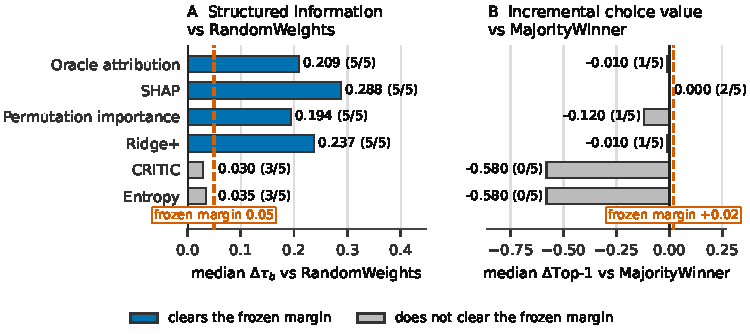
\includegraphics[width=\linewidth]{decision_value_figure}
\caption{Information learned is not decision value added. Left: every structured
method except \CRITIC{} and entropy clears the frozen $0.05$ Kendall margin against
RandomWeights. Right: no method reaches the frozen $+0.02$ Top-1 margin against the
constant MajorityWinner reference, and SHAP's advantage there is exactly zero. Both
panels are drawn directly from the frozen Pilot-B result on a common untruncated
scale.}
\label{fig:contrast}
\end{figure}

The exact oracle-attribution reference failed the same gate, so the stop cannot be
attributed to \XGB{} fitting error or TreeSHAP approximation alone.

\subsection{Post-Closure Descriptive Selection Maps}
\label{sec:selectionmaps}

The Pilot-B artefact retained aggregate metrics but not method-level context
selections. After permanent closure, a separate protocol was frozen before any
selection was reconstructed. It reused the archived fixed weights and TEST identities,
generated no target, fitted or queried no model, re-estimated no weight, and could not
alter the gate; an independent audit verified all $5\times7\times200=7000$ selections.
This is a post-closure descriptive diagnostic and has no confirmatory role.

Equal-weight \MOORA{} selected a single alternative in every context of every world and
matched MajorityWinner exactly in four of five worlds. Structured-method constancy was
heterogeneous, from zero worlds for PI to three for entropy
(Table~\ref{tab:selectionmaps}). The simple hypothesis that every fixed-weight \MOORA{}
vector must be context invariant is therefore not supported for the seven observed
vectors. World 21003 also shows why Top-1 and full-ranking fidelity must be reported
separately: Equal, \CRITIC{} and entropy all selected $A_6$ in all $200$ contexts,
giving identical Top-1 accuracy $0.190$ and mean regret $0.316758$, while their mean
$\tau_b$ values still differed ($0.5493$, $0.5427$, $0.5113$) because the lower ranks
differed. These observations suggest locally coarse decision regions for particular
fixed vectors. They do not characterize unobserved weight space, do not establish a
causal mechanism for the Pilot-B stop, and do not change its outcome.

\begin{table}[t]
\centering
\caption{Post-closure descriptive diagnostic over the seven observed fixed vectors.
Counts give worlds with a single selected alternative, and worlds with exact
context-level agreement with MajorityWinner. Descriptive only; non-confirmatory.}
\label{tab:selectionmaps}
\small
\begin{tabular}{@{}l@{\hspace{2em}}c@{\hspace{2em}}c@{}}
\toprule
Method & Constant-selection worlds & All-context MW-match worlds\\
\midrule
Oracle attribution & 1/5 & 1/5\\
SHAP & 2/5 & 2/5\\
Permutation importance & 0/5 & 0/5\\
Ridge+ & 1/5 & 1/5\\
CRITIC & 2/5 & 1/5\\
Entropy & 3/5 & 2/5\\
Equal & 5/5 & 4/5\\
\bottomrule
\end{tabular}
\end{table}

% ============================================================
\section{Discussion}
\label{sec:discussion}
% ============================================================

\subsection{What the Study Establishes}
\label{sec:establishes}

RQ1 and RQ2 are addressed by the prospectively structured benchmark-development and
Pilot-B evidence. The separately frozen post-closure diagnostic addresses DQ1
descriptively and has no confirmatory role.

For RQ1, an algebraic and numerical audit showed that contextual variation can vanish
entirely under the normalization used by the decision operator, and that a diagnostic
must be applied at that point to detect it. For RQ2, correcting exact separability
produced multiple oracle orderings and winners in every world, but it did not establish
sufficient incremental decision value: no structured global-weight pipeline escaped
MajorityWinner under the frozen cross-world rule.

The clearest reading is not that SHAP failed. Its separation from RandomWeights shows
that its weights carried reproducible ranking information, and that entire median
advantage then disappeared against a single constant choice: at this reference
condition the bottleneck lay in converting one global weight vector into
context-specific decision value through \MOORA{}. Because closed-form oracle
attribution reached the same outcome, an explanation resting solely on imperfect
learned attribution is ruled out. No single causal mechanism is isolated, however:
generator geometry, global compression, reference construction and \MOORA{} geometry
remain coupled in the executed design.

For applied OR and transport research the lesson is compact. A complex data-driven
pipeline should be compared not only against random or uniform parameters but also
against a meaningful simple decision policy: beating random weights shows that
information was learned, not that it usefully changes the operational choice.

\subsection{Interpretation Boundary and Limitations}
\label{sec:limits}

The central boundary statement is this. \emph{Pilot-B failure denotes failure of the
prespecified adequacy requirement for the intended global-weight--\MOORA{} comparison;
it does not imply that the generator contains no discriminative decision information.}
Four independent observations support the distinction: RandomWeights decisions were not
invariant; four structured methods separated from RandomWeights; SHAP held a large and
consistent Kendall advantage; and the observed fixed vectors displayed heterogeneous
selection constancy rather than uniform collapse. Equally, the result does not show
that SHAP universally fails, that global weights never matter, that \MOORA{} is
generally inadequate, that the D29 kernel is defective, that one ITS alternative is
best, or that MajorityWinner should be deployed.

Ten limitations bound the claim.

\begin{enumerate}
\itemsep1pt
\item Pilot B uses only five worlds, so cross-world inferential precision is low.
\item Those five are reused development worlds, not fresh ones.
\item Only one reference condition was evaluated, $(N,c,\rho,\lambda)=(250,0.30,0.4,0.5)$.
\item \emph{Prospective freezing prevents post-result modification of the gate, but it
does not make the five reused development worlds independent validation data.} The
result is a protocol-level adequacy screen; no population-level inference about method
performance is claimed.
\item MajorityWinner headroom varies strongly across worlds, from a modal share of
$0.519$ to $0.983$, so the difficulty of the comparison is itself heterogeneous.
\item MajorityWinner is Top-1-derived, not regret-optimal. The regret arm uses the same
prospectively frozen Top-1-derived constant reference rather than a separately
optimized regret-minimizing constant policy. A future benchmark could prospectively
define metric-matched constant references.
\item The generator, oracle and capability mask are synthetic assumptions, not
empirical transport effects, causal truth, stakeholder preferences or social welfare.
\item Every global-weight method intentionally compresses context-specific information,
and the methods differ in semantics: oracle attribution and SHAP target one
interventional functional; Ridge+ and PI use supervised association; \CRITIC{} and
entropy summarize pooled decision-matrix properties. PI can additionally extrapolate
when dependence is broken \cite{hooker2021permutation}.
\item The post-closure diagnostic adds no independent worlds. A paired context
bootstrap was prospectively excluded from that layer and was not executed; any
resampling study would require its own protocol and could not reopen the gate.
\item The paper makes no empirical ITS deployment recommendation.
\end{enumerate}

The negative result stays scientifically useful because it was not tuned away. The
generator correction, the gate thresholds, the evaluator and the seed firewall all
preceded the authorized result. Once the modal-winner stop fired, the 30-world primary
factorial and the reserve worlds remained barred. Any future design must begin as a
separately versioned study that discloses this closed result rather than retroactively
amending it.

% ============================================================
\section{Conclusion}
\label{sec:conclusion}
% ============================================================

This study asked whether a synthetic ITS benchmark could support a global XAI--MCDM
method comparison, and it asked before running the comparison at scale. Structural
auditing found and corrected a normalization-induced collapse in the original
generator, but that correction, while necessary, did not by itself establish downstream
decision discrimination. At the frozen development reference, four structured
methods---SHAP among them---cleared the RandomWeights adequacy criterion, yet none
cleared the MajorityWinner criterion, and closed-form oracle attribution failed the
same gate.

The defensible conclusion is narrow and actionable: at this reference condition the
evaluated global-weight-compression--\MOORA{} pipelines did not establish enough
incremental decision value to justify the protected primary factorial, and the gate
therefore performed its intended function. More broadly, synthetic XAI--MCDM studies
should validate not only prediction and attribution, but also whether the benchmark can
discriminate decisions beyond meaningful simple references. In XAI-assisted decision
support, recovering structured importance is not enough; the recovered information must
demonstrably change decisions in a useful way.

% ============================================================
\section*{Code and Data Availability}

The reproducibility package contains the synthetic benchmark generator, the frozen
configuration and protocol files, the deterministic seed definitions, the archived
development-audit and Pilot-B result artefacts, the frozen global-weight vectors, the
post-closure selection-map outputs, the independent audit and evaluator scripts, the
software-environment specification, content-integrity manifests, and the read-only
scripts that regenerate every table and figure reported here. Raw benchmark worlds are
regenerated deterministically from the frozen seeds and configurations rather than
stored as large duplicated datasets. Primary and reserve worlds were never accessed and
no primary result exists.
\ifanon
During double-blind review, identifying repository metadata is withheld; an anonymous
archive can be supplied to editors and reviewers on request. The complete
version-controlled repository and its immutable provenance record will be released
publicly after review.
\else
The complete version-controlled repository and its immutable provenance record are
released with the public reproducibility package.
\fi

\ifanon
\else
\section*{CRediT Authorship Contribution Statement}

\textbf{Mohamed Yassine Neifar:} Conceptualization, Methodology, Software, Validation,
Formal analysis, Investigation, Data curation, Visualization, Writing -- original
draft, Writing -- review and editing.
\textbf{Nadir Farhi:} Conceptualization, Methodology, Validation, Supervision,
Writing -- review and editing.
\textbf{Ahmed Frikha:} Supervision, Writing -- review and editing.
\fi

\section*{Funding}

This research did not receive any specific grant from funding agencies in the public,
commercial, or not-for-profit sectors.

\section*{Declaration of Competing Interest}

The authors declare that they have no known competing financial interests or personal
relationships that could have appeared to influence the work reported in this paper.

\section*{Declaration of Generative AI and AI-Assisted Technologies}

Generative AI tools were used for language editing, manuscript organization,
consistency checking and LaTeX assistance. All scientific design decisions, code
executions, numerical results, interpretations and citations were independently checked
by the authors, who take full responsibility for the manuscript.

\ifanon
\else
\section*{Acknowledgements}

The authors acknowledge the academic guidance and scientific support provided within
the doctoral research collaboration between the University of Sfax and Universit\'e
Gustave Eiffel.
\fi

% ============================================================
\begin{thebibliography}{99}

\bibitem{keeney1976decisions}
Keeney, R.L., Raiffa, H.:
Decisions with Multiple Objectives: Preferences and Value Tradeoffs.
Wiley, New York (1976).

\bibitem{roy1996importance}
Roy, B., Mousseau, V.:
A theoretical framework for analysing the notion of relative importance of criteria.
Journal of Multi-Criteria Decision Analysis \textbf{5}(2), 145--159 (1996).
\url{https://doi.org/10.1002/(SICI)1099-1360(199606)5:2<145::AID-MCDA99>3.0.CO;2-5}

\bibitem{choo1999weights}
Choo, E.U., Schoner, B., Wedley, W.C.:
Interpretation of criteria weights in multicriteria decision making.
Computers \& Industrial Engineering \textbf{37}(3), 527--541 (1999).
\url{https://doi.org/10.1016/S0360-8352(00)00019-X}

\bibitem{mukhametzyanov2021objective}
Mukhametzyanov, I.:
Specific character of objective methods for determining weights of criteria in MCDM
problems: Entropy, CRITIC and SD.
Decision Making: Applications in Management and Engineering \textbf{4}(2), 76--105
(2021).
\url{https://doi.org/10.31181/dmame210402076i}

\bibitem{chen2016xgboost}
Chen, T., Guestrin, C.:
XGBoost: A scalable tree boosting system.
In: Proceedings of the 22nd ACM SIGKDD International Conference on Knowledge Discovery
and Data Mining, pp. 785--794 (2016).
\url{https://doi.org/10.1145/2939672.2939785}

\bibitem{lundberg2017shap}
Lundberg, S.M., Lee, S.-I.:
A unified approach to interpreting model predictions.
In: Advances in Neural Information Processing Systems, vol. 30 (2017).

\bibitem{lundberg2020trees}
Lundberg, S.M., Erion, G., Chen, H., et al.:
From local explanations to global understanding with explainable AI for trees.
Nature Machine Intelligence \textbf{2}, 56--67 (2020).
\url{https://doi.org/10.1038/s42256-019-0138-9}

\bibitem{sundararajan2020many}
Sundararajan, M., Najmi, A.:
The many Shapley values for model explanation.
In: Proceedings of the 37th International Conference on Machine Learning,
PMLR \textbf{119}, 9269--9278 (2020).

\bibitem{kumar2020shapleyproblems}
Kumar, I.E., Venkatasubramanian, S., Scheidegger, C., Friedler, S.:
Problems with Shapley-value-based explanations as feature importance measures.
In: Proceedings of the 37th International Conference on Machine Learning,
PMLR \textbf{119}, 5491--5500 (2020).

\bibitem{janzing2020causal}
Janzing, D., Minorics, L., Bl{\"o}baum, P.:
Feature relevance quantification in explainable AI: A causal problem.
In: Proceedings of the 23rd International Conference on Artificial Intelligence and
Statistics, PMLR \textbf{108}, 2907--2916 (2020).

\bibitem{hooker2021permutation}
Hooker, G., Mentch, L., Zhou, S.:
Unrestricted permutation forces extrapolation: Variable importance requires at least
one more model, or there is no free variable importance.
Statistics and Computing \textbf{31}, 82 (2021).
\url{https://doi.org/10.1007/s11222-021-10057-z}

\bibitem{liu2021xaibench}
Liu, Y., Khandagale, S., White, C., Neiswanger, W.:
Synthetic benchmarks for scientific research in explainable machine learning.
Proceedings of the Neural Information Processing Systems Track on Datasets and
Benchmarks \textbf{1} (2021).

\bibitem{agarwal2022openxai}
Agarwal, C., Krishna, S., Saxena, E., Pawelczyk, M., Johnson, N., Puri, I., Zitnik, M.,
Lakkaraju, H.:
OpenXAI: Towards a transparent evaluation of model explanations.
In: Advances in Neural Information Processing Systems, vol. 35, Datasets and Benchmarks
Track (2022).

\bibitem{ciano2025xaimcdm}
Ciano, T., Ferrara, M.:
Explainable multi-criteria decision making for tourism economics: Integrating XAI with
MCDM for a robust accommodation performance assessment.
Decisions in Economics and Finance (2025).
\url{https://doi.org/10.1007/s10203-025-00553-6}

\bibitem{demir2025shapmultimoora}
Demir, A.S., Da{\u g}deviren, U., Kurnaz, T.F., Erden, C., K{\"o}k{\c c}am, A.H.:
An integrated SHAP-MCDM approach for slope stability prediction based on machine
learning algorithms.
Natural Hazards \textbf{121}(18), 21811--21836 (2025).
\url{https://doi.org/10.1007/s11069-025-07665-7}

\bibitem{zakeri2024mlmcdm}
Zakeri, S., Konstantas, D., Sorooshian, S., Chatterjee, P.:
A novel ML-MCDM-based decision support system for evaluating autonomous vehicle
integration scenarios in Geneva's public transportation.
Artificial Intelligence Review \textbf{57}, 310 (2024).
\url{https://doi.org/10.1007/s10462-024-10917-w}

\bibitem{diakoulaki1995critic}
Diakoulaki, D., Mavrotas, G., Papayannakis, L.:
Determining objective weights in multiple criteria problems: The CRITIC method.
Computers \& Operations Research \textbf{22}(7), 763--770 (1995).
\url{https://doi.org/10.1016/0305-0548(94)00059-H}

\bibitem{shannon1948}
Shannon, C.E.:
A mathematical theory of communication.
Bell System Technical Journal \textbf{27}, 379--423, 623--656 (1948).

\bibitem{brauers2006moora}
Brauers, W.K.M., Zavadskas, E.K.:
The MOORA method and its application to privatization in a transition economy.
Control and Cybernetics \textbf{35}(2), 445--469 (2006).

\bibitem{fhwa2016corridors}
Federal Highway Administration:
Planning for Transportation Systems Management and Operations Within Corridors: A Desk
Reference, FHWA-HOP-16-037 (2016).
\url{https://ops.fhwa.dot.gov/Publications/fhwahop16037/}

\bibitem{fhwa2017atm}
Kuhn, B., Balke, K., Wood, N.:
Active Traffic Management (ATM) Implementation and Operations Guide.
FHWA-HOP-17-056, Federal Highway Administration (2017).
\url{https://ops.fhwa.dot.gov/publications/fhwahop17056/}

\bibitem{usdotv2x}
U.S. Department of Transportation, ITS Joint Program Office:
V2X Applications and Use Cases.
\url{https://its.dot.gov/research-areas/V2X-Deployment/overview/v2x-applications/}
(accessed 13 August 2026).

\bibitem{morris2019simulation}
Morris, T.P., White, I.R., Crowther, M.J.:
Using simulation studies to evaluate statistical methods.
Statistics in Medicine \textbf{38}(11), 2074--2102 (2019).
\url{https://doi.org/10.1002/sim.8086}

\bibitem{niessl2022overoptimism}
Nie{\ss}l, C., Herrmann, M., Wiedemann, C., Casalicchio, G., Boulesteix, A.-L.:
Over-optimism in benchmark studies and the multiplicity of design and analysis options
when interpreting their results.
WIREs Data Mining and Knowledge Discovery \textbf{12}(2), e1441 (2022).
\url{https://doi.org/10.1002/widm.1441}

\end{thebibliography}

\end{document}
"
%
% No numerical result in this file may be edited by hand. Every reported value
% is verified against the frozen artefacts by
%   scripts/paper/verify_frozen_manuscript_numbers.py
% ============================================================
% ChkTeX: intentional en dashes, citation spacing, label placement, acronym
% punctuation and LNCS bibliography conventions.
% chktex-file 2
% chktex-file 8
% chktex-file 13
% chktex-file 24
% chktex-file 36

\documentclass[runningheads,orivec]{llncs}

\usepackage[T1]{fontenc}
\usepackage[utf8]{inputenc}
\usepackage{amsmath,amssymb,amsfonts}
\usepackage{booktabs}
\usepackage{tabularx}
\usepackage{graphicx}
\usepackage{tikz}
\usetikzlibrary{arrows.meta,positioning,calc}
\usepackage{hyperref}

\hypersetup{hidelinks}
\graphicspath{{../outputs/paper/figures/}{./figures/}{./}}

% ---- build-mode switch: anonymous by default -----------------
\providecommand{\CAMERAREADY}{0}
\newif\ifanon
\anontrue
\ifnum\CAMERAREADY=1 \anonfalse \fi
% --------------------------------------------------------------

\newcommand{\XGB}{XGBoost}
\newcommand{\MOORA}{MOORA}
\newcommand{\CRITIC}{CRITIC}
\newcommand{\E}{\mathbb{E}}

\begin{document}
\emergencystretch=1.5em

\title{From Predictive Importance to Decision Value: Evaluating XAI-Based
Weights for ITS Prioritisation}
\titlerunning{From Predictive Importance to Decision Value}

\ifanon
  \author{Anonymous Author(s)}
  \authorrunning{Anonymous Author(s)}
  \institute{Anonymous Institution(s)}
\else
  \author{Mohamed Yassine Neifar\inst{1,2}\thanks{Corresponding author.} \and
  Ahmed Frikha\inst{2} \and
  Nadir Farhi\inst{1}}
  \authorrunning{Neifar et al.}
  \institute{Universit\'e Gustave Eiffel, COSYS--GRETTIA,
  14--20 Boulevard Newton, Cit\'e Descartes, Champs-sur-Marne,
  F-77447 Marne-la-Vall\'ee Cedex 2, France
  \and
  Institut Sup\'erieur de Gestion Industrielle de Sfax (ISGIS),
  OLID, University of Sfax, Route de l'A\'eroport km 4, BP 1099,
  Sfax 3038, Tunisia\\
  \email{yessine.neifar.imsil@isgis.usf.tn}}
\fi

\maketitle

\begin{abstract}
Feature attributions from predictive models are increasingly rescaled into global
criterion weights for multi-criteria decision-making. Predictive importance and
decision value are, however, different quantities, and a benchmark must be able to
tell them apart before it can compare methods. We build a controlled synthetic
laboratory for Intelligent Transportation Systems prioritisation: six alternatives,
ten criteria, a nonlinear oracle, \XGB, interventional TreeSHAP, six structured
global-weight pipelines and benefit-oriented \MOORA. A structural audit first showed
that the original generator's apparent contextual variation cancelled exactly under
the normalization used by the decision operator. A corrected monotone response kernel
removed that algebraic collapse. We then executed a five-world adequacy gate that had
been frozen before execution. Four structured methods, including SHAP, cleared the
prospectively specified RandomWeights adequacy criterion; SHAP reached a median
Kendall $\tau_b$ improvement of $0.288$, positive in all five worlds. No structured
method cleared the MajorityWinner criterion---SHAP's median Top-1 and regret
advantages against that constant reference were exactly zero---and closed-form oracle
attribution failed the same gate, so the outcome is not an artefact of learned
approximation. The gate therefore stopped the protected primary factorial. Recovering
structured importance is not sufficient: synthetic XAI--MCDM benchmarks should
demonstrate incremental decision value against meaningful simple references before
comparing methods.

\keywords{Explainable AI \and Multi-Criteria Decision-Making \and Benchmark Validity
\and Prospective Stopping \and Decision Support \and Intelligent Transportation
Systems}
\end{abstract}

% ============================================================
\section{Introduction}
\label{sec:introduction}
% ============================================================

Transport agencies routinely prioritise Intelligent Transportation Systems (ITS) with
limited operational evidence and limited capacity for formal preference elicitation.
The task is naturally multi-criteria: candidate deployments differ in mobility,
reliability, person-throughput, safety, environmental performance, accessibility,
readiness, interoperability and lifecycle burden. Machine learning and explainable
artificial intelligence (XAI) offer an attractive shortcut. Fit a performance model,
aggregate its feature attributions into criterion ``importance'', normalize the result
into weights, and rank alternatives with a multi-criteria decision-making (MCDM) rule.

That shortcut contains a semantic leap and an empirical one. MCDM weights take their
meaning from criterion scales and from the aggregation model; they are not generic
measures of importance \cite{keeney1976decisions,roy1996importance,choo1999weights}.
SHAP values allocate model output under a specified cooperative-game functional
\cite{lundberg2017shap}, but a predictive attribution is not automatically a
stakeholder preference, a causal effect or a valid trade-off constant
\cite{sundararajan2020many,kumar2020shapleyproblems,janzing2020causal}. Consequently
\[
\text{predictive attribution}
\;\longrightarrow\;
\text{global criterion weight}
\;\longrightarrow\;
\text{MCDM ranking}
\]
is a pipeline to be validated, not an identity to be assumed.

Controlled synthetic studies look well suited to that validation, because the
data-generating process and an oracle reference are both known. Yet a synthetic
benchmark can carry a great deal of raw variation and still pose a nearly trivial
decision problem, and a method comparison run on such a benchmark measures
implementation differences rather than decision value. Benchmark studies are also
vulnerable to over-optimism when generators, estimands or analyses are revised after
method performance has been observed
\cite{morris2019simulation,niessl2022overoptimism}.

We therefore separate two notions and use them consistently throughout.
\emph{Validity} refers to the conceptual scientific properties of the benchmark:
whether its responses vary, whether that variation survives normalization, whether the
oracle is well defined. \emph{Adequacy} refers to the operational, prospectively frozen
test used to decide whether a protected primary comparison is warranted at all. A
benchmark can be valid and still be inadequate.

We address two prospective research questions.

\begin{description}
\item[RQ1.] Can structural diagnostics reveal when apparent contextual variation
disappears under the normalization used by the downstream MCDM operator?
\item[RQ2.] After correcting that structural defect, do structured global-weight
pipelines provide sufficient incremental decision value over random-weight and
constant-decision references to justify protected primary evaluation?
\end{description}

After the study was permanently closed we additionally froze one descriptive
diagnostic, reported here under a deliberately separate label.

\begin{description}
\item[DQ1 (post-closure, descriptive).] After Pilot B was permanently closed, what do
the archived context-level selection maps reveal about the observed decision behaviour
of the seven frozen fixed-weight vectors?
\end{description}

DQ1 is post-closure and descriptive. It is non-confirmatory, and it cannot modify,
reinterpret or reopen the Pilot-B gate. It is reported because it is explanatory, not
because it carries evidential weight.

The paper contributes a validation workflow rather than a new weighting algorithm. It
separates raw variation, structural non-separability and downstream decision
discrimination and shows that the first two do not imply the third; it carries a
closed-form oracle attribution alongside learned SHAP, separating estimation error
from losses created by global compression and aggregation; and it demonstrates a
prospectively frozen adequacy gate that stops a planned comparison when its decision
premise fails. To our knowledge this is a rare prospectively gated controlled
evaluation of whether global attribution-derived weights retain downstream decision
value after MCDM aggregation. The generator genealogy, candidate grids, seed
namespaces, software tests, frozen protocols and unexecuted analyses are preserved in
the companion supplement.

Figure~\ref{fig:workflow} gives the study logic end to end. Three features are
central: estimation data and external TEST contexts are disjoint, an oracle reference
runs in parallel with the learned pipeline, and the final gate is evaluated before the
protected experiment is allowed to start.

\begin{figure}[t]
\centering
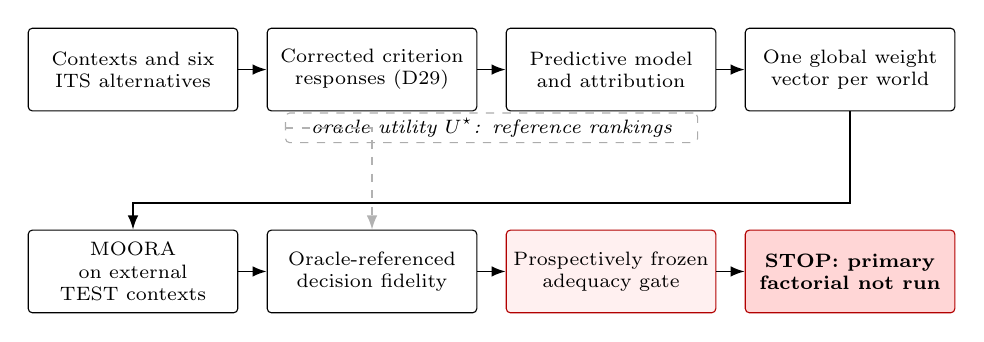
\begin{tikzpicture}[
  node distance=3.2mm and 3.6mm,
  box/.style={draw, rounded corners=1.5pt, align=center, minimum height=10.5mm,
              text width=.205\linewidth, inner sep=2.5pt, font=\scriptsize},
  gate/.style={draw=red!70!black, fill=red!6, rounded corners=1.5pt, align=center,
               minimum height=10.5mm, text width=.205\linewidth, inner sep=2.5pt,
               font=\scriptsize},
  stop/.style={draw=red!70!black, fill=red!16, rounded corners=1.5pt, align=center,
               minimum height=10.5mm, text width=.205\linewidth, inner sep=2.5pt,
               font=\scriptsize\bfseries},
  oracle/.style={draw=gray!65, dashed, rounded corners=1.5pt, align=center,
                 text width=.42\linewidth, inner sep=2pt, font=\scriptsize\itshape},
  arr/.style={-{Latex[length=1.8mm]}, semithick}
]
\node[box] (ctx)  {Contexts and six\\ITS alternatives};
\node[box, right=of ctx]  (resp) {Corrected criterion\\responses (D29)};
\node[box, right=of resp] (attr) {Predictive model\\and attribution};
\node[box, right=of attr] (wts)  {One global weight\\vector per world};

\node[box, below=15mm of ctx]  (moora) {\MOORA{} on external\\TEST contexts};
\node[box, right=of moora] (fid)   {Oracle-referenced\\decision fidelity};
\node[gate, right=of fid]  (gatee) {Prospectively frozen\\adequacy gate};
\node[stop, right=of gatee] (stopn) {STOP: primary\\factorial not run};

\draw[arr] (ctx)  -- (resp);
\draw[arr] (resp) -- (attr);
\draw[arr] (attr) -- (wts);
\draw[arr] (wts.south) -- ++(0,-11.6mm) -| ([xshift=0mm]moora.north);
\draw[arr] (moora) -- (fid);
\draw[arr] (fid)   -- (gatee);
\draw[arr] (gatee) -- (stopn);
% The oracle runs alongside the learned pipeline and supplies the reference
% rankings that decision fidelity is scored against.
\node[oracle] (orc) at ($(resp)!0.5!(attr) + (0,-7.4mm)$)
  {oracle utility $U^\star$: reference rankings};
\draw[arr,dashed,gray!60] (orc.west) -| (fid.north);
\end{tikzpicture}
\caption{Study logic. Estimation partitions (FIT and WEIGHT) support model fitting and
global-weight estimation; disjoint external TEST contexts support \MOORA{} decisions
and oracle-referenced fidelity. The gate decides whether the protected primary
comparison is scientifically warranted; here it decided against.}
\label{fig:workflow}
\end{figure}

% ============================================================
\section{Related Work and Contribution Boundary}
\label{sec:related}
% ============================================================

XAI--MCDM studies have shown that model explanations can be integrated with ranking
methods across domains including transport and infrastructure
\cite{ciano2025xaimcdm,demir2025shapmultimoora,zakeri2024mlmcdm}, while objective
weighting methods such as \CRITIC{} and entropy derive weights from dispersion and
conflict within a decision matrix
\cite{diakoulaki1995critic,shannon1948,mukhametzyanov2021objective}. These families
answer different questions: attribution summarizes a predictive functional, regression
and permutation summarize supervised association, and objective weights summarize the
observed criterion matrix. Their outputs are numerically comparable but are not
interchangeable notions of preference.

Synthetic XAI benchmarks typically compare explanations against known attribution
targets \cite{liu2021xaibench,agarwal2022openxai}. Our focus lies one step downstream.
Even exact recovery of a global attribution functional need not recover
context-specific oracle choices once that functional has been compressed into a single
fixed weight vector and passed through an aggregation rule. Prediction, attribution and
decision fidelity can fail at different stages, so we evaluate learned SHAP alongside a
matched closed-form oracle attribution using ranking, Top-1 and regret metrics.

The contribution boundary is deliberately narrow. This study does not estimate
empirical ITS effects, does not elicit stakeholder preferences, does not identify a
preferred real-world intervention, and does not test whether SHAP works in general. ITS
supplies a controlled applied decision setting. The scientific object is the adequacy
of a global-weight XAI--MCDM benchmark at one prospectively specified development
reference condition.

% ============================================================
\section{Benchmark and Validation Design}
\label{sec:methods}
% ============================================================

\subsection{An ITS Decision Laboratory}
\label{sec:lab}

The benchmark compares six deployment packages at a common first-stage prioritisation
level (Table~\ref{tab:alternatives}). They represent deployable ITS and
transport-systems-management families rather than city-specific calibrated effects
\cite{fhwa2016corridors,fhwa2017atm,usdotv2x}.

\begin{table}[t]
\centering
\caption{ITS alternatives in the controlled decision laboratory.}
\label{tab:alternatives}
\small
\begin{tabularx}{\linewidth}{@{}c l X@{}}
\toprule
\textbf{ID} & \textbf{Alternative} & \textbf{Operational scope}\\
\midrule
$A_1$ & ATSC & Adaptive phase, split, offset or cycle decisions.\\
$A_2$ & TSP & Transit-priority requests and signal responses.\\
$A_3$ & TIDM & Incident detection, verification, response and recovery.\\
$A_4$ & RMTI--DRG & Real-time multimodal information and dynamic route guidance.\\
$A_5$ & V2X--CS & Cooperative safety warnings, excluding signal timing and TSP.\\
$A_6$ & DSM & Dynamic speed management and harmonisation.\\
\bottomrule
\end{tabularx}
\end{table}

Ten benefit-oriented criteria cover mobility efficiency, reliability,
person-throughput, safety, resilience, environmental efficiency, accessibility,
readiness, interoperability/scalability and direction-adjusted lifecycle burden, driven
by five correlated latent factors: demand, incidents, person movement, environmental
sensitivity and infrastructure readiness.

\emph{Each replication seed defines one benchmark world}: its technology parameters,
its contexts and all of its random streams. The world is the statistical unit
throughout this paper. Alternative--context rows are never treated as independent
population replications.

\subsection{A Structural Defect and the D29 Correction}
\label{sec:generator}

The initial noise-free response for the seven active criteria $C_1$--$C_7$ had the form
\begin{equation}
g_{asj}=\theta_{aj}\,o_{sj},
\label{eq:separable}
\end{equation}
where $a$, $s$ and $j$ index alternative, context and criterion, $\theta_{aj}$ is a
capability amplitude and $o_{sj}$ a context opportunity. Under the vector
normalization used by the decision operator, for $o_{sj}>0$,
\begin{equation}
r_{asj}
=\frac{\theta_{aj}o_{sj}}{\sqrt{\sum_b\theta_{bj}^2o_{sj}^2}}
=\frac{\theta_{aj}}{\sqrt{\sum_b\theta_{bj}^2}}.
\label{eq:collapse}
\end{equation}
The common opportunity term cancels exactly, so every context yields an identical
normalized column. Sum, max and min--max normalizations exhibit the same common-scale
cancellation. This answers RQ1: raw contextual variation, on its own, was not evidence
that the benchmark posed a context-sensitive decision problem, and only a diagnostic
applied \emph{at the operator's normalization} could reveal it.

After prospectively separated calibration and eligibility screening, the frozen
correction---referred to as the D29 kernel---for the active $C_1$--$C_7$ pathways was
\begin{equation}
g_{asj}=\theta_{aj}o_{sj}+0.05\,v_{aj}\,o_{sj}(1-o_{sj}),
\qquad v_{aj}\in[-1,1].
\label{eq:d29}
\end{equation}
The deterministic contrast values $v_{aj}$ were assigned without any outcome or winner
information. Because active $\theta_{aj}\ge0.05$, the response stays monotone on
$o\in[0,1]$. D29 was retained for protocol continuity and minimal intervention among
$54$ corrected-eligible candidates, not because it produced a preferred ITS winner or a
favourable method comparison. The rejected families and the full candidate history are
supplementary.

\subsection{Oracle, Global Weights and the Decision Operator}
\label{sec:oracle}

Benefit-oriented criterion values are passed through $q_j(g)=\log(1+2g)/\log 3$. The
noise-free oracle utility is
\begin{equation}
U_{as}^{\star}
=\frac{\sum_{j=1}^{10}\alpha_j q_j(g_{asj})
+\lambda\sum_{(j,k)\in\mathcal E}0.20\,q_j(g_{asj})q_k(g_{ask})}
{1+\lambda}.
\label{eq:oracle}
\end{equation}
This is an internally specified reference, not causal truth and not social welfare.
The prediction target adds controlled noise to $U^\star$. Because
Eq.~\eqref{eq:oracle} contains only main effects and pairwise interactions, the frozen
interventional Shapley functional admits a closed-form \emph{oracle attribution}.
Global oracle weights normalize mean absolute WEIGHT-set attributions; learned SHAP
applies the same aggregation to interventional TreeSHAP values from a fixed \XGB{}
model \cite{chen2016xgboost,lundberg2020trees}.

Six structured global-weight methods enter the gate: oracle attribution, SHAP,
fixed-model context-block permutation importance (PI), non-negative Ridge+, \CRITIC{}
and entropy. Equal, RandomWeights and MajorityWinner serve as diagnostic references.
Every weighting method produces exactly one context-invariant vector per world, which
is the point: the design deliberately asks what survives that compression. Estimation
uses disjoint FIT and WEIGHT partitions, and the $200$ external TEST contexts are never
used for fitting or weight estimation. At the Pilot-B size $N=250$, each world holds
$200$ FIT, $50$ WEIGHT and $200$ TEST contexts.

The downstream operator is benefit-oriented weighted \MOORA{} \cite{brauers2006moora}:
\begin{equation}
r_{asj}=\frac{g_{asj}}{\sqrt{\sum_{b=1}^{6}g_{bsj}^2}+10^{-12}},
\qquad
S_{as}=\sum_{j=1}^{10}w_j r_{asj}.
\label{eq:moora}
\end{equation}
Alternatives are ranked by descending $S_{as}$. All score representations use an
absolute $10^{-12}$ tie tolerance, anchor-based average ranks without tie chaining, and
ascending alternative ID for deterministic Top-1 selection.

\subsection{Decision Fidelity and the Prospective Adequacy Gate}
\label{sec:gate}

Agreement with the oracle is measured three ways: full-ranking agreement by Kendall's
$\tau_b$, deterministic Top-1 accuracy, and normalized oracle regret
\begin{equation}
R_s^{(q)}=
\frac{U_{a_s^\star,s}^{\star}-U_{\hat a_s^{(q)},s}^{\star}}
{\max_a U_{as}^{\star}-\min_a U_{as}^{\star}+10^{-12}}.
\label{eq:regret}
\end{equation}

Pilot B was frozen before execution at $(N,c,\rho,\lambda)=(250,0.30,0.4,0.5)$ over
development worlds 21001--21005. It uses $200$ common
$\operatorname{Dirichlet}(1,\ldots,1)$ RandomWeights draws per world and one
MajorityWinner per world.

MajorityWinner is an oracle-informed diagnostic reference. It is the context-free
oracle-modal alternative estimated on WEIGHT and evaluated on TEST---the constant
alternative maximizing empirical oracle Top-1 frequency on WEIGHT. It is not claimed to
minimize regret or to constitute an operational transportation policy, and it is
neither stakeholder-derived nor normative. It is included precisely because it is
strong and cheap: a global-weight pipeline should add decision value beyond a single
constant choice before its additional complexity is considered justified.

A practical method advantage must be strictly positive in at least four of the five
worlds \emph{and} meet the relevant cross-world median margin.
Table~\ref{tab:gates} lists the five independently sufficient stop conditions. The
overall rule is an OR: the benchmark passes only if every stop is false. The margins
are design-specific adequacy tolerances, not universal equivalence bounds.

\begin{table}[t]
\centering
\caption{The five prospectively frozen Pilot-B stop conditions. Any one of them halts
the study; passage requires all five to be false.}
\label{tab:gates}
\small
\begin{tabularx}{\linewidth}{@{}l X@{}}
\toprule
\textbf{Stop} & \textbf{Condition}\\
\midrule
Coverage & A required structured output or RandomWeights coverage is missing.\\
Random equivalence & No method clears median $\Delta\tau_b=0.05$ or
$\Delta$mean-regret $=0.01$ versus RandomWeights.\\
Modal-winner tie & No method clears median $\Delta$Top-1 $=0.02$ or
$\Delta$mean-regret $=0.01$ versus MajorityWinner.\\
Oracle dominance & Pooled oracle modal share is at least $0.90$.\\
Weight insensitivity & Random-weight choices or performance widths meet the frozen
invariance criteria.\\
\bottomrule
\end{tabularx}
\end{table}

The protocol, the evaluator and the protected-seed firewall were committed before the
single authorized execution. A 30-world, 135-cell primary factorial and its associated
robustness analyses were conditional on Pilot-B passage. They were not run. This is
version-controlled prospective specification rather than public preregistration; the
complete provenance appears in the supplement.

% ============================================================
\section{Results}
\label{sec:results}
% ============================================================

\subsection{Structural Validity Did Not Guarantee Decision Diversity}
\label{sec:structural}

The historical generator of Eq.~\eqref{eq:separable} collapsed numerically exactly
where the algebra predicted. Across all $35$ world--criterion combinations the maximum
active-pair log-ratio variation was $7.2224\times10^{-16}$ and the maximum
vector-normalized profile variation was $1.8036\times10^{-9}$: machine noise, not
signal.

The corrected D29 kernel cleared the frozen structural and reachability requirements,
and it did produce multiple oracle orderings and multiple oracle winners in every
world---between $17$ and $78$ distinct complete orderings and between two and five
distinct winners. Yet its oracle decision geometry stayed markedly uneven. The modal
oracle winner's share ranged from $0.519$ to $0.983$ across the five worlds, with a
median of $0.809$. In world 21001, the directly comparable case, the correction raised
the number of distinct oracle orderings from $19$ to $23$ while also raising modal
share from $0.962$ to $0.983$.

Removing exact multiplicative separability was therefore necessary for this benchmark
but not sufficient. In three of five worlds a single alternative was already
oracle-optimal in over $80\%$ of contexts, which sets a high bar for any pipeline that
must beat a constant choice.

\subsection{The Pilot-B Result}
\label{sec:pilotb}

All six structured methods were defined in every world, every required Kendall summary
was available, and no Equal fallback was used. Table~\ref{tab:gateoutcome} reports the
independently reconstructed gate decision. Four of six methods separated from
RandomWeights, so the random-equivalence stop was false. The pooled oracle modal share
was $0.526$ ($A_2$ in $526$ of $1000$ TEST contexts), so no single alternative
dominated the pooled worlds, and RandomWeights decisions were not invariant. Exactly
one stop fired: the modal-winner effective tie.

\begin{table}[t]
\centering
\caption{Frozen Pilot-B outcome. The overall hard stop is the OR of the five flags;
one flag fired.}
\label{tab:gateoutcome}
\small
\begin{tabularx}{\linewidth}{@{}lXc@{}}
\toprule
Gate & Audited result & Stop\\
\midrule
Coverage & Six structured methods eligible without fallback & No\\
Random equivalence & Four of six methods separated from RandomWeights & No\\
Modal-winner tie & Zero of six methods escaped MajorityWinner & \textbf{Yes}\\
Oracle dominance & Pooled modal share $0.526<0.90$ & No\\
Weight insensitivity & Invariant fraction $0.004<0.90$; qualified worlds $0<4$ & No\\
\midrule
Overall & At least one prospectively frozen stop fired & \textbf{Yes}\\
\bottomrule
\end{tabularx}
\end{table}

Table~\ref{tab:contrasts} and Fig.~\ref{fig:contrast} localize the failure; positive
values favour the structured method. Oracle attribution, SHAP, PI and Ridge+ each
cleared a RandomWeights criterion with the required cross-world consistency. SHAP
showed the largest median Kendall improvement, $0.288$, positive in all five worlds,
together with a median regret improvement of $0.026060$, positive in four. Against
MajorityWinner, by contrast, SHAP's median Top-1 and median regret advantages were both
exactly zero, with only two positive worlds. No method met either modal-winner margin
with the required four-of-five consistency.

The compact statement of the whole result is this. \emph{Four structured methods,
including SHAP, cleared the prospectively specified RandomWeights adequacy criterion,
but no structured method cleared the prospectively specified MajorityWinner adequacy
criterion.}

\begin{table}[t]
\centering
\caption{Cross-world median Pilot-B contrasts, with the count of strictly positive
worlds in parentheses (P, out of five). MW denotes MajorityWinner, RW RandomWeights.
The last column reports the frozen RandomWeights separation verdict.}
\label{tab:contrasts}
\scriptsize
\setlength{\tabcolsep}{2.5pt}
\begin{tabular}{@{}lrrrrc@{}}
\toprule
Method & \shortstack{MW\\$\Delta$Top-1 (P)} & \shortstack{MW\\$\Delta$regret (P)} &
\shortstack{RW\\$\Delta\tau_b$ (P)} & \shortstack{RW\\$\Delta$regret (P)} & RW sep.\\
\midrule
Oracle attribution & $-0.010$ (1) & $-0.002119$ (1) & $0.209$ (5) & $0.023940$ (4) & Yes\\
SHAP & $0.000$ (2) & $0.000000$ (2) & $0.288$ (5) & $0.026060$ (4) & Yes\\
Permutation importance & $-0.120$ (1) & $-0.004425$ (1) & $0.194$ (5) & $0.010658$ (4) & Yes\\
Ridge+ & $-0.010$ (1) & $-0.002119$ (1) & $0.237$ (5) & $0.011492$ (4) & Yes\\
CRITIC & $-0.580$ (0) & $-0.124414$ (0) & $0.030$ (3) & $-0.098354$ (0) & No\\
Entropy & $-0.580$ (0) & $-0.156641$ (0) & $0.035$ (3) & $-0.002807$ (1) & No\\
\bottomrule
\end{tabular}
\end{table}

\begin{figure}[t]
\centering
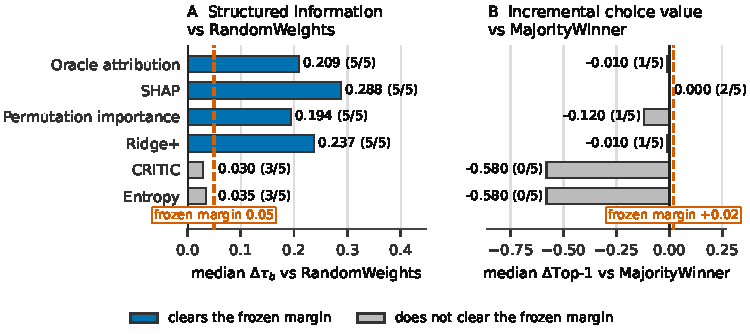
\includegraphics[width=\linewidth]{decision_value_figure}
\caption{Information learned is not decision value added. Left: every structured
method except \CRITIC{} and entropy clears the frozen $0.05$ Kendall margin against
RandomWeights. Right: no method reaches the frozen $+0.02$ Top-1 margin against the
constant MajorityWinner reference, and SHAP's advantage there is exactly zero. Both
panels are drawn directly from the frozen Pilot-B result on a common untruncated
scale.}
\label{fig:contrast}
\end{figure}

The exact oracle-attribution reference failed the same gate, so the stop cannot be
attributed to \XGB{} fitting error or TreeSHAP approximation alone.

\subsection{Post-Closure Descriptive Selection Maps}
\label{sec:selectionmaps}

The Pilot-B artefact retained aggregate metrics but not method-level context
selections. After permanent closure, a separate protocol was frozen before any
selection was reconstructed. It reused the archived fixed weights and TEST identities,
generated no target, fitted or queried no model, re-estimated no weight, and could not
alter the gate; an independent audit verified all $5\times7\times200=7000$ selections.
This is a post-closure descriptive diagnostic and has no confirmatory role.

Equal-weight \MOORA{} selected a single alternative in every context of every world and
matched MajorityWinner exactly in four of five worlds. Structured-method constancy was
heterogeneous, from zero worlds for PI to three for entropy
(Table~\ref{tab:selectionmaps}). The simple hypothesis that every fixed-weight \MOORA{}
vector must be context invariant is therefore not supported for the seven observed
vectors. World 21003 also shows why Top-1 and full-ranking fidelity must be reported
separately: Equal, \CRITIC{} and entropy all selected $A_6$ in all $200$ contexts,
giving identical Top-1 accuracy $0.190$ and mean regret $0.316758$, while their mean
$\tau_b$ values still differed ($0.5493$, $0.5427$, $0.5113$) because the lower ranks
differed. These observations suggest locally coarse decision regions for particular
fixed vectors. They do not characterize unobserved weight space, do not establish a
causal mechanism for the Pilot-B stop, and do not change its outcome.

\begin{table}[t]
\centering
\caption{Post-closure descriptive diagnostic over the seven observed fixed vectors.
Counts give worlds with a single selected alternative, and worlds with exact
context-level agreement with MajorityWinner. Descriptive only; non-confirmatory.}
\label{tab:selectionmaps}
\small
\begin{tabular}{@{}l@{\hspace{2em}}c@{\hspace{2em}}c@{}}
\toprule
Method & Constant-selection worlds & All-context MW-match worlds\\
\midrule
Oracle attribution & 1/5 & 1/5\\
SHAP & 2/5 & 2/5\\
Permutation importance & 0/5 & 0/5\\
Ridge+ & 1/5 & 1/5\\
CRITIC & 2/5 & 1/5\\
Entropy & 3/5 & 2/5\\
Equal & 5/5 & 4/5\\
\bottomrule
\end{tabular}
\end{table}

% ============================================================
\section{Discussion}
\label{sec:discussion}
% ============================================================

\subsection{What the Study Establishes}
\label{sec:establishes}

RQ1 and RQ2 are addressed by the prospectively structured benchmark-development and
Pilot-B evidence. The separately frozen post-closure diagnostic addresses DQ1
descriptively and has no confirmatory role.

For RQ1, an algebraic and numerical audit showed that contextual variation can vanish
entirely under the normalization used by the decision operator, and that a diagnostic
must be applied at that point to detect it. For RQ2, correcting exact separability
produced multiple oracle orderings and winners in every world, but it did not establish
sufficient incremental decision value: no structured global-weight pipeline escaped
MajorityWinner under the frozen cross-world rule.

The clearest reading is not that SHAP failed. Its separation from RandomWeights shows
that its weights carried reproducible ranking information, and that entire median
advantage then disappeared against a single constant choice: at this reference
condition the bottleneck lay in converting one global weight vector into
context-specific decision value through \MOORA{}. Because closed-form oracle
attribution reached the same outcome, an explanation resting solely on imperfect
learned attribution is ruled out. No single causal mechanism is isolated, however:
generator geometry, global compression, reference construction and \MOORA{} geometry
remain coupled in the executed design.

For applied OR and transport research the lesson is compact. A complex data-driven
pipeline should be compared not only against random or uniform parameters but also
against a meaningful simple decision policy: beating random weights shows that
information was learned, not that it usefully changes the operational choice.

\subsection{Interpretation Boundary and Limitations}
\label{sec:limits}

The central boundary statement is this. \emph{Pilot-B failure denotes failure of the
prespecified adequacy requirement for the intended global-weight--\MOORA{} comparison;
it does not imply that the generator contains no discriminative decision information.}
Four independent observations support the distinction: RandomWeights decisions were not
invariant; four structured methods separated from RandomWeights; SHAP held a large and
consistent Kendall advantage; and the observed fixed vectors displayed heterogeneous
selection constancy rather than uniform collapse. Equally, the result does not show
that SHAP universally fails, that global weights never matter, that \MOORA{} is
generally inadequate, that the D29 kernel is defective, that one ITS alternative is
best, or that MajorityWinner should be deployed.

Ten limitations bound the claim.

\begin{enumerate}
\itemsep1pt
\item Pilot B uses only five worlds, so cross-world inferential precision is low.
\item Those five are reused development worlds, not fresh ones.
\item Only one reference condition was evaluated, $(N,c,\rho,\lambda)=(250,0.30,0.4,0.5)$.
\item \emph{Prospective freezing prevents post-result modification of the gate, but it
does not make the five reused development worlds independent validation data.} The
result is a protocol-level adequacy screen; no population-level inference about method
performance is claimed.
\item MajorityWinner headroom varies strongly across worlds, from a modal share of
$0.519$ to $0.983$, so the difficulty of the comparison is itself heterogeneous.
\item MajorityWinner is Top-1-derived, not regret-optimal. The regret arm uses the same
prospectively frozen Top-1-derived constant reference rather than a separately
optimized regret-minimizing constant policy. A future benchmark could prospectively
define metric-matched constant references.
\item The generator, oracle and capability mask are synthetic assumptions, not
empirical transport effects, causal truth, stakeholder preferences or social welfare.
\item Every global-weight method intentionally compresses context-specific information,
and the methods differ in semantics: oracle attribution and SHAP target one
interventional functional; Ridge+ and PI use supervised association; \CRITIC{} and
entropy summarize pooled decision-matrix properties. PI can additionally extrapolate
when dependence is broken \cite{hooker2021permutation}.
\item The post-closure diagnostic adds no independent worlds. A paired context
bootstrap was prospectively excluded from that layer and was not executed; any
resampling study would require its own protocol and could not reopen the gate.
\item The paper makes no empirical ITS deployment recommendation.
\end{enumerate}

The negative result stays scientifically useful because it was not tuned away. The
generator correction, the gate thresholds, the evaluator and the seed firewall all
preceded the authorized result. Once the modal-winner stop fired, the 30-world primary
factorial and the reserve worlds remained barred. Any future design must begin as a
separately versioned study that discloses this closed result rather than retroactively
amending it.

% ============================================================
\section{Conclusion}
\label{sec:conclusion}
% ============================================================

This study asked whether a synthetic ITS benchmark could support a global XAI--MCDM
method comparison, and it asked before running the comparison at scale. Structural
auditing found and corrected a normalization-induced collapse in the original
generator, but that correction, while necessary, did not by itself establish downstream
decision discrimination. At the frozen development reference, four structured
methods---SHAP among them---cleared the RandomWeights adequacy criterion, yet none
cleared the MajorityWinner criterion, and closed-form oracle attribution failed the
same gate.

The defensible conclusion is narrow and actionable: at this reference condition the
evaluated global-weight-compression--\MOORA{} pipelines did not establish enough
incremental decision value to justify the protected primary factorial, and the gate
therefore performed its intended function. More broadly, synthetic XAI--MCDM studies
should validate not only prediction and attribution, but also whether the benchmark can
discriminate decisions beyond meaningful simple references. In XAI-assisted decision
support, recovering structured importance is not enough; the recovered information must
demonstrably change decisions in a useful way.

% ============================================================
\section*{Code and Data Availability}

The reproducibility package contains the synthetic benchmark generator, the frozen
configuration and protocol files, the deterministic seed definitions, the archived
development-audit and Pilot-B result artefacts, the frozen global-weight vectors, the
post-closure selection-map outputs, the independent audit and evaluator scripts, the
software-environment specification, content-integrity manifests, and the read-only
scripts that regenerate every table and figure reported here. Raw benchmark worlds are
regenerated deterministically from the frozen seeds and configurations rather than
stored as large duplicated datasets. Primary and reserve worlds were never accessed and
no primary result exists.
\ifanon
During double-blind review, identifying repository metadata is withheld; an anonymous
archive can be supplied to editors and reviewers on request. The complete
version-controlled repository and its immutable provenance record will be released
publicly after review.
\else
The complete version-controlled repository and its immutable provenance record are
released with the public reproducibility package.
\fi

\ifanon
\else
\section*{CRediT Authorship Contribution Statement}

\textbf{Mohamed Yassine Neifar:} Conceptualization, Methodology, Software, Validation,
Formal analysis, Investigation, Data curation, Visualization, Writing -- original
draft, Writing -- review and editing.
\textbf{Nadir Farhi:} Conceptualization, Methodology, Validation, Supervision,
Writing -- review and editing.
\textbf{Ahmed Frikha:} Supervision, Writing -- review and editing.
\fi

\section*{Funding}

This research did not receive any specific grant from funding agencies in the public,
commercial, or not-for-profit sectors.

\section*{Declaration of Competing Interest}

The authors declare that they have no known competing financial interests or personal
relationships that could have appeared to influence the work reported in this paper.

\section*{Declaration of Generative AI and AI-Assisted Technologies}

Generative AI tools were used for language editing, manuscript organization,
consistency checking and LaTeX assistance. All scientific design decisions, code
executions, numerical results, interpretations and citations were independently checked
by the authors, who take full responsibility for the manuscript.

\ifanon
\else
\section*{Acknowledgements}

The authors acknowledge the academic guidance and scientific support provided within
the doctoral research collaboration between the University of Sfax and Universit\'e
Gustave Eiffel.
\fi

% ============================================================
\begin{thebibliography}{99}

\bibitem{keeney1976decisions}
Keeney, R.L., Raiffa, H.:
Decisions with Multiple Objectives: Preferences and Value Tradeoffs.
Wiley, New York (1976).

\bibitem{roy1996importance}
Roy, B., Mousseau, V.:
A theoretical framework for analysing the notion of relative importance of criteria.
Journal of Multi-Criteria Decision Analysis \textbf{5}(2), 145--159 (1996).
\url{https://doi.org/10.1002/(SICI)1099-1360(199606)5:2<145::AID-MCDA99>3.0.CO;2-5}

\bibitem{choo1999weights}
Choo, E.U., Schoner, B., Wedley, W.C.:
Interpretation of criteria weights in multicriteria decision making.
Computers \& Industrial Engineering \textbf{37}(3), 527--541 (1999).
\url{https://doi.org/10.1016/S0360-8352(00)00019-X}

\bibitem{mukhametzyanov2021objective}
Mukhametzyanov, I.:
Specific character of objective methods for determining weights of criteria in MCDM
problems: Entropy, CRITIC and SD.
Decision Making: Applications in Management and Engineering \textbf{4}(2), 76--105
(2021).
\url{https://doi.org/10.31181/dmame210402076i}

\bibitem{chen2016xgboost}
Chen, T., Guestrin, C.:
XGBoost: A scalable tree boosting system.
In: Proceedings of the 22nd ACM SIGKDD International Conference on Knowledge Discovery
and Data Mining, pp. 785--794 (2016).
\url{https://doi.org/10.1145/2939672.2939785}

\bibitem{lundberg2017shap}
Lundberg, S.M., Lee, S.-I.:
A unified approach to interpreting model predictions.
In: Advances in Neural Information Processing Systems, vol. 30 (2017).

\bibitem{lundberg2020trees}
Lundberg, S.M., Erion, G., Chen, H., et al.:
From local explanations to global understanding with explainable AI for trees.
Nature Machine Intelligence \textbf{2}, 56--67 (2020).
\url{https://doi.org/10.1038/s42256-019-0138-9}

\bibitem{sundararajan2020many}
Sundararajan, M., Najmi, A.:
The many Shapley values for model explanation.
In: Proceedings of the 37th International Conference on Machine Learning,
PMLR \textbf{119}, 9269--9278 (2020).

\bibitem{kumar2020shapleyproblems}
Kumar, I.E., Venkatasubramanian, S., Scheidegger, C., Friedler, S.:
Problems with Shapley-value-based explanations as feature importance measures.
In: Proceedings of the 37th International Conference on Machine Learning,
PMLR \textbf{119}, 5491--5500 (2020).

\bibitem{janzing2020causal}
Janzing, D., Minorics, L., Bl{\"o}baum, P.:
Feature relevance quantification in explainable AI: A causal problem.
In: Proceedings of the 23rd International Conference on Artificial Intelligence and
Statistics, PMLR \textbf{108}, 2907--2916 (2020).

\bibitem{hooker2021permutation}
Hooker, G., Mentch, L., Zhou, S.:
Unrestricted permutation forces extrapolation: Variable importance requires at least
one more model, or there is no free variable importance.
Statistics and Computing \textbf{31}, 82 (2021).
\url{https://doi.org/10.1007/s11222-021-10057-z}

\bibitem{liu2021xaibench}
Liu, Y., Khandagale, S., White, C., Neiswanger, W.:
Synthetic benchmarks for scientific research in explainable machine learning.
Proceedings of the Neural Information Processing Systems Track on Datasets and
Benchmarks \textbf{1} (2021).

\bibitem{agarwal2022openxai}
Agarwal, C., Krishna, S., Saxena, E., Pawelczyk, M., Johnson, N., Puri, I., Zitnik, M.,
Lakkaraju, H.:
OpenXAI: Towards a transparent evaluation of model explanations.
In: Advances in Neural Information Processing Systems, vol. 35, Datasets and Benchmarks
Track (2022).

\bibitem{ciano2025xaimcdm}
Ciano, T., Ferrara, M.:
Explainable multi-criteria decision making for tourism economics: Integrating XAI with
MCDM for a robust accommodation performance assessment.
Decisions in Economics and Finance (2025).
\url{https://doi.org/10.1007/s10203-025-00553-6}

\bibitem{demir2025shapmultimoora}
Demir, A.S., Da{\u g}deviren, U., Kurnaz, T.F., Erden, C., K{\"o}k{\c c}am, A.H.:
An integrated SHAP-MCDM approach for slope stability prediction based on machine
learning algorithms.
Natural Hazards \textbf{121}(18), 21811--21836 (2025).
\url{https://doi.org/10.1007/s11069-025-07665-7}

\bibitem{zakeri2024mlmcdm}
Zakeri, S., Konstantas, D., Sorooshian, S., Chatterjee, P.:
A novel ML-MCDM-based decision support system for evaluating autonomous vehicle
integration scenarios in Geneva's public transportation.
Artificial Intelligence Review \textbf{57}, 310 (2024).
\url{https://doi.org/10.1007/s10462-024-10917-w}

\bibitem{diakoulaki1995critic}
Diakoulaki, D., Mavrotas, G., Papayannakis, L.:
Determining objective weights in multiple criteria problems: The CRITIC method.
Computers \& Operations Research \textbf{22}(7), 763--770 (1995).
\url{https://doi.org/10.1016/0305-0548(94)00059-H}

\bibitem{shannon1948}
Shannon, C.E.:
A mathematical theory of communication.
Bell System Technical Journal \textbf{27}, 379--423, 623--656 (1948).

\bibitem{brauers2006moora}
Brauers, W.K.M., Zavadskas, E.K.:
The MOORA method and its application to privatization in a transition economy.
Control and Cybernetics \textbf{35}(2), 445--469 (2006).

\bibitem{fhwa2016corridors}
Federal Highway Administration:
Planning for Transportation Systems Management and Operations Within Corridors: A Desk
Reference, FHWA-HOP-16-037 (2016).
\url{https://ops.fhwa.dot.gov/Publications/fhwahop16037/}

\bibitem{fhwa2017atm}
Kuhn, B., Balke, K., Wood, N.:
Active Traffic Management (ATM) Implementation and Operations Guide.
FHWA-HOP-17-056, Federal Highway Administration (2017).
\url{https://ops.fhwa.dot.gov/publications/fhwahop17056/}

\bibitem{usdotv2x}
U.S. Department of Transportation, ITS Joint Program Office:
V2X Applications and Use Cases.
\url{https://its.dot.gov/research-areas/V2X-Deployment/overview/v2x-applications/}
(accessed 13 August 2026).

\bibitem{morris2019simulation}
Morris, T.P., White, I.R., Crowther, M.J.:
Using simulation studies to evaluate statistical methods.
Statistics in Medicine \textbf{38}(11), 2074--2102 (2019).
\url{https://doi.org/10.1002/sim.8086}

\bibitem{niessl2022overoptimism}
Nie{\ss}l, C., Herrmann, M., Wiedemann, C., Casalicchio, G., Boulesteix, A.-L.:
Over-optimism in benchmark studies and the multiplicity of design and analysis options
when interpreting their results.
WIREs Data Mining and Knowledge Discovery \textbf{12}(2), e1441 (2022).
\url{https://doi.org/10.1002/widm.1441}

\end{thebibliography}

\end{document}
"
%
% No numerical result in this file may be edited by hand. Every reported value
% is verified against the frozen artefacts by
%   scripts/paper/verify_frozen_manuscript_numbers.py
% ============================================================
% ChkTeX: intentional en dashes, citation spacing, label placement, acronym
% punctuation and LNCS bibliography conventions.
% chktex-file 2
% chktex-file 8
% chktex-file 13
% chktex-file 24
% chktex-file 36

\documentclass[runningheads,orivec]{llncs}

\usepackage[T1]{fontenc}
\usepackage[utf8]{inputenc}
\usepackage{amsmath,amssymb,amsfonts}
\usepackage{booktabs}
\usepackage{tabularx}
\usepackage{graphicx}
\usepackage{tikz}
\usetikzlibrary{arrows.meta,positioning,calc}
\usepackage{hyperref}

\hypersetup{hidelinks}
\graphicspath{{../outputs/paper/figures/}{./figures/}{./}}

% ---- build-mode switch: anonymous by default -----------------
\providecommand{\CAMERAREADY}{0}
\newif\ifanon
\anontrue
\ifnum\CAMERAREADY=1 \anonfalse \fi
% --------------------------------------------------------------

\newcommand{\XGB}{XGBoost}
\newcommand{\MOORA}{MOORA}
\newcommand{\CRITIC}{CRITIC}
\newcommand{\E}{\mathbb{E}}

\begin{document}
\emergencystretch=1.5em

\title{From Predictive Importance to Decision Value: Evaluating XAI-Based
Weights for ITS Prioritisation}
\titlerunning{From Predictive Importance to Decision Value}

\ifanon
  \author{Anonymous Author(s)}
  \authorrunning{Anonymous Author(s)}
  \institute{Anonymous Institution(s)}
\else
  \author{Mohamed Yassine Neifar\inst{1,2}\thanks{Corresponding author.} \and
  Ahmed Frikha\inst{2} \and
  Nadir Farhi\inst{1}}
  \authorrunning{Neifar et al.}
  \institute{Universit\'e Gustave Eiffel, COSYS--GRETTIA,
  14--20 Boulevard Newton, Cit\'e Descartes, Champs-sur-Marne,
  F-77447 Marne-la-Vall\'ee Cedex 2, France
  \and
  Institut Sup\'erieur de Gestion Industrielle de Sfax (ISGIS),
  OLID, University of Sfax, Route de l'A\'eroport km 4, BP 1099,
  Sfax 3038, Tunisia\\
  \email{yessine.neifar.imsil@isgis.usf.tn}}
\fi

\maketitle

\begin{abstract}
Feature attributions from predictive models are increasingly rescaled into global
criterion weights for multi-criteria decision-making. Predictive importance and
decision value are, however, different quantities, and a benchmark must be able to
tell them apart before it can compare methods. We build a controlled synthetic
laboratory for Intelligent Transportation Systems prioritisation: six alternatives,
ten criteria, a nonlinear oracle, \XGB, interventional TreeSHAP, six structured
global-weight pipelines and benefit-oriented \MOORA. A structural audit first showed
that the original generator's apparent contextual variation cancelled exactly under
the normalization used by the decision operator. A corrected monotone response kernel
removed that algebraic collapse. We then executed a five-world adequacy gate that had
been frozen before execution. Four structured methods, including SHAP, cleared the
prospectively specified RandomWeights adequacy criterion; SHAP reached a median
Kendall $\tau_b$ improvement of $0.288$, positive in all five worlds. No structured
method cleared the MajorityWinner criterion---SHAP's median Top-1 and regret
advantages against that constant reference were exactly zero---and closed-form oracle
attribution failed the same gate, so the outcome is not an artefact of learned
approximation. The gate therefore stopped the protected primary factorial. Recovering
structured importance is not sufficient: synthetic XAI--MCDM benchmarks should
demonstrate incremental decision value against meaningful simple references before
comparing methods.

\keywords{Explainable AI \and Multi-Criteria Decision-Making \and Benchmark Validity
\and Prospective Stopping \and Decision Support \and Intelligent Transportation
Systems}
\end{abstract}

% ============================================================
\section{Introduction}
\label{sec:introduction}
% ============================================================

Transport agencies routinely prioritise Intelligent Transportation Systems (ITS) with
limited operational evidence and limited capacity for formal preference elicitation.
The task is naturally multi-criteria: candidate deployments differ in mobility,
reliability, person-throughput, safety, environmental performance, accessibility,
readiness, interoperability and lifecycle burden. Machine learning and explainable
artificial intelligence (XAI) offer an attractive shortcut. Fit a performance model,
aggregate its feature attributions into criterion ``importance'', normalize the result
into weights, and rank alternatives with a multi-criteria decision-making (MCDM) rule.

That shortcut contains a semantic leap and an empirical one. MCDM weights take their
meaning from criterion scales and from the aggregation model; they are not generic
measures of importance \cite{keeney1976decisions,roy1996importance,choo1999weights}.
SHAP values allocate model output under a specified cooperative-game functional
\cite{lundberg2017shap}, but a predictive attribution is not automatically a
stakeholder preference, a causal effect or a valid trade-off constant
\cite{sundararajan2020many,kumar2020shapleyproblems,janzing2020causal}. Consequently
\[
\text{predictive attribution}
\;\longrightarrow\;
\text{global criterion weight}
\;\longrightarrow\;
\text{MCDM ranking}
\]
is a pipeline to be validated, not an identity to be assumed.

Controlled synthetic studies look well suited to that validation, because the
data-generating process and an oracle reference are both known. Yet a synthetic
benchmark can carry a great deal of raw variation and still pose a nearly trivial
decision problem, and a method comparison run on such a benchmark measures
implementation differences rather than decision value. Benchmark studies are also
vulnerable to over-optimism when generators, estimands or analyses are revised after
method performance has been observed
\cite{morris2019simulation,niessl2022overoptimism}.

We therefore separate two notions and use them consistently throughout.
\emph{Validity} refers to the conceptual scientific properties of the benchmark:
whether its responses vary, whether that variation survives normalization, whether the
oracle is well defined. \emph{Adequacy} refers to the operational, prospectively frozen
test used to decide whether a protected primary comparison is warranted at all. A
benchmark can be valid and still be inadequate.

We address two prospective research questions.

\begin{description}
\item[RQ1.] Can structural diagnostics reveal when apparent contextual variation
disappears under the normalization used by the downstream MCDM operator?
\item[RQ2.] After correcting that structural defect, do structured global-weight
pipelines provide sufficient incremental decision value over random-weight and
constant-decision references to justify protected primary evaluation?
\end{description}

After the study was permanently closed we additionally froze one descriptive
diagnostic, reported here under a deliberately separate label.

\begin{description}
\item[DQ1 (post-closure, descriptive).] After Pilot B was permanently closed, what do
the archived context-level selection maps reveal about the observed decision behaviour
of the seven frozen fixed-weight vectors?
\end{description}

DQ1 is post-closure and descriptive. It is non-confirmatory, and it cannot modify,
reinterpret or reopen the Pilot-B gate. It is reported because it is explanatory, not
because it carries evidential weight.

The paper contributes a validation workflow rather than a new weighting algorithm. It
separates raw variation, structural non-separability and downstream decision
discrimination and shows that the first two do not imply the third; it carries a
closed-form oracle attribution alongside learned SHAP, separating estimation error
from losses created by global compression and aggregation; and it demonstrates a
prospectively frozen adequacy gate that stops a planned comparison when its decision
premise fails. To our knowledge this is a rare prospectively gated controlled
evaluation of whether global attribution-derived weights retain downstream decision
value after MCDM aggregation. The generator genealogy, candidate grids, seed
namespaces, software tests, frozen protocols and unexecuted analyses are preserved in
the companion supplement.

Figure~\ref{fig:workflow} gives the study logic end to end. Three features are
central: estimation data and external TEST contexts are disjoint, an oracle reference
runs in parallel with the learned pipeline, and the final gate is evaluated before the
protected experiment is allowed to start.

\begin{figure}[t]
\centering
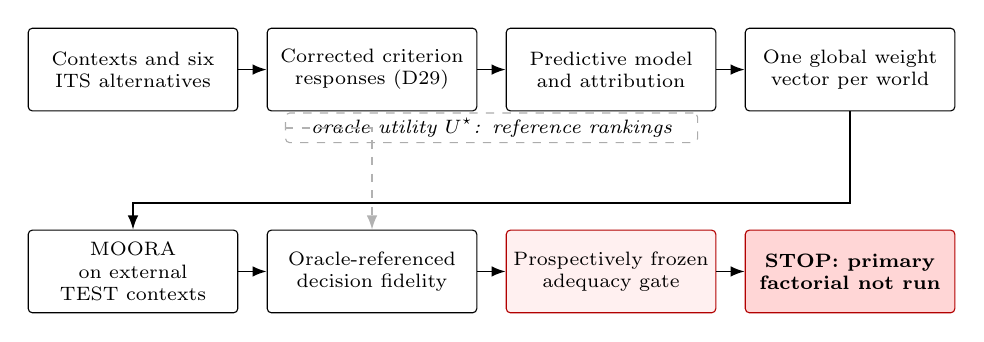
\begin{tikzpicture}[
  node distance=3.2mm and 3.6mm,
  box/.style={draw, rounded corners=1.5pt, align=center, minimum height=10.5mm,
              text width=.205\linewidth, inner sep=2.5pt, font=\scriptsize},
  gate/.style={draw=red!70!black, fill=red!6, rounded corners=1.5pt, align=center,
               minimum height=10.5mm, text width=.205\linewidth, inner sep=2.5pt,
               font=\scriptsize},
  stop/.style={draw=red!70!black, fill=red!16, rounded corners=1.5pt, align=center,
               minimum height=10.5mm, text width=.205\linewidth, inner sep=2.5pt,
               font=\scriptsize\bfseries},
  oracle/.style={draw=gray!65, dashed, rounded corners=1.5pt, align=center,
                 text width=.42\linewidth, inner sep=2pt, font=\scriptsize\itshape},
  arr/.style={-{Latex[length=1.8mm]}, semithick}
]
\node[box] (ctx)  {Contexts and six\\ITS alternatives};
\node[box, right=of ctx]  (resp) {Corrected criterion\\responses (D29)};
\node[box, right=of resp] (attr) {Predictive model\\and attribution};
\node[box, right=of attr] (wts)  {One global weight\\vector per world};

\node[box, below=15mm of ctx]  (moora) {\MOORA{} on external\\TEST contexts};
\node[box, right=of moora] (fid)   {Oracle-referenced\\decision fidelity};
\node[gate, right=of fid]  (gatee) {Prospectively frozen\\adequacy gate};
\node[stop, right=of gatee] (stopn) {STOP: primary\\factorial not run};

\draw[arr] (ctx)  -- (resp);
\draw[arr] (resp) -- (attr);
\draw[arr] (attr) -- (wts);
\draw[arr] (wts.south) -- ++(0,-11.6mm) -| ([xshift=0mm]moora.north);
\draw[arr] (moora) -- (fid);
\draw[arr] (fid)   -- (gatee);
\draw[arr] (gatee) -- (stopn);
% The oracle runs alongside the learned pipeline and supplies the reference
% rankings that decision fidelity is scored against.
\node[oracle] (orc) at ($(resp)!0.5!(attr) + (0,-7.4mm)$)
  {oracle utility $U^\star$: reference rankings};
\draw[arr,dashed,gray!60] (orc.west) -| (fid.north);
\end{tikzpicture}
\caption{Study logic. Estimation partitions (FIT and WEIGHT) support model fitting and
global-weight estimation; disjoint external TEST contexts support \MOORA{} decisions
and oracle-referenced fidelity. The gate decides whether the protected primary
comparison is scientifically warranted; here it decided against.}
\label{fig:workflow}
\end{figure}

% ============================================================
\section{Related Work and Contribution Boundary}
\label{sec:related}
% ============================================================

XAI--MCDM studies have shown that model explanations can be integrated with ranking
methods across domains including transport and infrastructure
\cite{ciano2025xaimcdm,demir2025shapmultimoora,zakeri2024mlmcdm}, while objective
weighting methods such as \CRITIC{} and entropy derive weights from dispersion and
conflict within a decision matrix
\cite{diakoulaki1995critic,shannon1948,mukhametzyanov2021objective}. These families
answer different questions: attribution summarizes a predictive functional, regression
and permutation summarize supervised association, and objective weights summarize the
observed criterion matrix. Their outputs are numerically comparable but are not
interchangeable notions of preference.

Synthetic XAI benchmarks typically compare explanations against known attribution
targets \cite{liu2021xaibench,agarwal2022openxai}. Our focus lies one step downstream.
Even exact recovery of a global attribution functional need not recover
context-specific oracle choices once that functional has been compressed into a single
fixed weight vector and passed through an aggregation rule. Prediction, attribution and
decision fidelity can fail at different stages, so we evaluate learned SHAP alongside a
matched closed-form oracle attribution using ranking, Top-1 and regret metrics.

The contribution boundary is deliberately narrow. This study does not estimate
empirical ITS effects, does not elicit stakeholder preferences, does not identify a
preferred real-world intervention, and does not test whether SHAP works in general. ITS
supplies a controlled applied decision setting. The scientific object is the adequacy
of a global-weight XAI--MCDM benchmark at one prospectively specified development
reference condition.

% ============================================================
\section{Benchmark and Validation Design}
\label{sec:methods}
% ============================================================

\subsection{An ITS Decision Laboratory}
\label{sec:lab}

The benchmark compares six deployment packages at a common first-stage prioritisation
level (Table~\ref{tab:alternatives}). They represent deployable ITS and
transport-systems-management families rather than city-specific calibrated effects
\cite{fhwa2016corridors,fhwa2017atm,usdotv2x}.

\begin{table}[t]
\centering
\caption{ITS alternatives in the controlled decision laboratory.}
\label{tab:alternatives}
\small
\begin{tabularx}{\linewidth}{@{}c l X@{}}
\toprule
\textbf{ID} & \textbf{Alternative} & \textbf{Operational scope}\\
\midrule
$A_1$ & ATSC & Adaptive phase, split, offset or cycle decisions.\\
$A_2$ & TSP & Transit-priority requests and signal responses.\\
$A_3$ & TIDM & Incident detection, verification, response and recovery.\\
$A_4$ & RMTI--DRG & Real-time multimodal information and dynamic route guidance.\\
$A_5$ & V2X--CS & Cooperative safety warnings, excluding signal timing and TSP.\\
$A_6$ & DSM & Dynamic speed management and harmonisation.\\
\bottomrule
\end{tabularx}
\end{table}

Ten benefit-oriented criteria cover mobility efficiency, reliability,
person-throughput, safety, resilience, environmental efficiency, accessibility,
readiness, interoperability/scalability and direction-adjusted lifecycle burden, driven
by five correlated latent factors: demand, incidents, person movement, environmental
sensitivity and infrastructure readiness.

\emph{Each replication seed defines one benchmark world}: its technology parameters,
its contexts and all of its random streams. The world is the statistical unit
throughout this paper. Alternative--context rows are never treated as independent
population replications.

\subsection{A Structural Defect and the D29 Correction}
\label{sec:generator}

The initial noise-free response for the seven active criteria $C_1$--$C_7$ had the form
\begin{equation}
g_{asj}=\theta_{aj}\,o_{sj},
\label{eq:separable}
\end{equation}
where $a$, $s$ and $j$ index alternative, context and criterion, $\theta_{aj}$ is a
capability amplitude and $o_{sj}$ a context opportunity. Under the vector
normalization used by the decision operator, for $o_{sj}>0$,
\begin{equation}
r_{asj}
=\frac{\theta_{aj}o_{sj}}{\sqrt{\sum_b\theta_{bj}^2o_{sj}^2}}
=\frac{\theta_{aj}}{\sqrt{\sum_b\theta_{bj}^2}}.
\label{eq:collapse}
\end{equation}
The common opportunity term cancels exactly, so every context yields an identical
normalized column. Sum, max and min--max normalizations exhibit the same common-scale
cancellation. This answers RQ1: raw contextual variation, on its own, was not evidence
that the benchmark posed a context-sensitive decision problem, and only a diagnostic
applied \emph{at the operator's normalization} could reveal it.

After prospectively separated calibration and eligibility screening, the frozen
correction---referred to as the D29 kernel---for the active $C_1$--$C_7$ pathways was
\begin{equation}
g_{asj}=\theta_{aj}o_{sj}+0.05\,v_{aj}\,o_{sj}(1-o_{sj}),
\qquad v_{aj}\in[-1,1].
\label{eq:d29}
\end{equation}
The deterministic contrast values $v_{aj}$ were assigned without any outcome or winner
information. Because active $\theta_{aj}\ge0.05$, the response stays monotone on
$o\in[0,1]$. D29 was retained for protocol continuity and minimal intervention among
$54$ corrected-eligible candidates, not because it produced a preferred ITS winner or a
favourable method comparison. The rejected families and the full candidate history are
supplementary.

\subsection{Oracle, Global Weights and the Decision Operator}
\label{sec:oracle}

Benefit-oriented criterion values are passed through $q_j(g)=\log(1+2g)/\log 3$. The
noise-free oracle utility is
\begin{equation}
U_{as}^{\star}
=\frac{\sum_{j=1}^{10}\alpha_j q_j(g_{asj})
+\lambda\sum_{(j,k)\in\mathcal E}0.20\,q_j(g_{asj})q_k(g_{ask})}
{1+\lambda}.
\label{eq:oracle}
\end{equation}
This is an internally specified reference, not causal truth and not social welfare.
The prediction target adds controlled noise to $U^\star$. Because
Eq.~\eqref{eq:oracle} contains only main effects and pairwise interactions, the frozen
interventional Shapley functional admits a closed-form \emph{oracle attribution}.
Global oracle weights normalize mean absolute WEIGHT-set attributions; learned SHAP
applies the same aggregation to interventional TreeSHAP values from a fixed \XGB{}
model \cite{chen2016xgboost,lundberg2020trees}.

Six structured global-weight methods enter the gate: oracle attribution, SHAP,
fixed-model context-block permutation importance (PI), non-negative Ridge+, \CRITIC{}
and entropy. Equal, RandomWeights and MajorityWinner serve as diagnostic references.
Every weighting method produces exactly one context-invariant vector per world, which
is the point: the design deliberately asks what survives that compression. Estimation
uses disjoint FIT and WEIGHT partitions, and the $200$ external TEST contexts are never
used for fitting or weight estimation. At the Pilot-B size $N=250$, each world holds
$200$ FIT, $50$ WEIGHT and $200$ TEST contexts.

The downstream operator is benefit-oriented weighted \MOORA{} \cite{brauers2006moora}:
\begin{equation}
r_{asj}=\frac{g_{asj}}{\sqrt{\sum_{b=1}^{6}g_{bsj}^2}+10^{-12}},
\qquad
S_{as}=\sum_{j=1}^{10}w_j r_{asj}.
\label{eq:moora}
\end{equation}
Alternatives are ranked by descending $S_{as}$. All score representations use an
absolute $10^{-12}$ tie tolerance, anchor-based average ranks without tie chaining, and
ascending alternative ID for deterministic Top-1 selection.

\subsection{Decision Fidelity and the Prospective Adequacy Gate}
\label{sec:gate}

Agreement with the oracle is measured three ways: full-ranking agreement by Kendall's
$\tau_b$, deterministic Top-1 accuracy, and normalized oracle regret
\begin{equation}
R_s^{(q)}=
\frac{U_{a_s^\star,s}^{\star}-U_{\hat a_s^{(q)},s}^{\star}}
{\max_a U_{as}^{\star}-\min_a U_{as}^{\star}+10^{-12}}.
\label{eq:regret}
\end{equation}

Pilot B was frozen before execution at $(N,c,\rho,\lambda)=(250,0.30,0.4,0.5)$ over
development worlds 21001--21005. It uses $200$ common
$\operatorname{Dirichlet}(1,\ldots,1)$ RandomWeights draws per world and one
MajorityWinner per world.

MajorityWinner is an oracle-informed diagnostic reference. It is the context-free
oracle-modal alternative estimated on WEIGHT and evaluated on TEST---the constant
alternative maximizing empirical oracle Top-1 frequency on WEIGHT. It is not claimed to
minimize regret or to constitute an operational transportation policy, and it is
neither stakeholder-derived nor normative. It is included precisely because it is
strong and cheap: a global-weight pipeline should add decision value beyond a single
constant choice before its additional complexity is considered justified.

A practical method advantage must be strictly positive in at least four of the five
worlds \emph{and} meet the relevant cross-world median margin.
Table~\ref{tab:gates} lists the five independently sufficient stop conditions. The
overall rule is an OR: the benchmark passes only if every stop is false. The margins
are design-specific adequacy tolerances, not universal equivalence bounds.

\begin{table}[t]
\centering
\caption{The five prospectively frozen Pilot-B stop conditions. Any one of them halts
the study; passage requires all five to be false.}
\label{tab:gates}
\small
\begin{tabularx}{\linewidth}{@{}l X@{}}
\toprule
\textbf{Stop} & \textbf{Condition}\\
\midrule
Coverage & A required structured output or RandomWeights coverage is missing.\\
Random equivalence & No method clears median $\Delta\tau_b=0.05$ or
$\Delta$mean-regret $=0.01$ versus RandomWeights.\\
Modal-winner tie & No method clears median $\Delta$Top-1 $=0.02$ or
$\Delta$mean-regret $=0.01$ versus MajorityWinner.\\
Oracle dominance & Pooled oracle modal share is at least $0.90$.\\
Weight insensitivity & Random-weight choices or performance widths meet the frozen
invariance criteria.\\
\bottomrule
\end{tabularx}
\end{table}

The protocol, the evaluator and the protected-seed firewall were committed before the
single authorized execution. A 30-world, 135-cell primary factorial and its associated
robustness analyses were conditional on Pilot-B passage. They were not run. This is
version-controlled prospective specification rather than public preregistration; the
complete provenance appears in the supplement.

% ============================================================
\section{Results}
\label{sec:results}
% ============================================================

\subsection{Structural Validity Did Not Guarantee Decision Diversity}
\label{sec:structural}

The historical generator of Eq.~\eqref{eq:separable} collapsed numerically exactly
where the algebra predicted. Across all $35$ world--criterion combinations the maximum
active-pair log-ratio variation was $7.2224\times10^{-16}$ and the maximum
vector-normalized profile variation was $1.8036\times10^{-9}$: machine noise, not
signal.

The corrected D29 kernel cleared the frozen structural and reachability requirements,
and it did produce multiple oracle orderings and multiple oracle winners in every
world---between $17$ and $78$ distinct complete orderings and between two and five
distinct winners. Yet its oracle decision geometry stayed markedly uneven. The modal
oracle winner's share ranged from $0.519$ to $0.983$ across the five worlds, with a
median of $0.809$. In world 21001, the directly comparable case, the correction raised
the number of distinct oracle orderings from $19$ to $23$ while also raising modal
share from $0.962$ to $0.983$.

Removing exact multiplicative separability was therefore necessary for this benchmark
but not sufficient. In three of five worlds a single alternative was already
oracle-optimal in over $80\%$ of contexts, which sets a high bar for any pipeline that
must beat a constant choice.

\subsection{The Pilot-B Result}
\label{sec:pilotb}

All six structured methods were defined in every world, every required Kendall summary
was available, and no Equal fallback was used. Table~\ref{tab:gateoutcome} reports the
independently reconstructed gate decision. Four of six methods separated from
RandomWeights, so the random-equivalence stop was false. The pooled oracle modal share
was $0.526$ ($A_2$ in $526$ of $1000$ TEST contexts), so no single alternative
dominated the pooled worlds, and RandomWeights decisions were not invariant. Exactly
one stop fired: the modal-winner effective tie.

\begin{table}[t]
\centering
\caption{Frozen Pilot-B outcome. The overall hard stop is the OR of the five flags;
one flag fired.}
\label{tab:gateoutcome}
\small
\begin{tabularx}{\linewidth}{@{}lXc@{}}
\toprule
Gate & Audited result & Stop\\
\midrule
Coverage & Six structured methods eligible without fallback & No\\
Random equivalence & Four of six methods separated from RandomWeights & No\\
Modal-winner tie & Zero of six methods escaped MajorityWinner & \textbf{Yes}\\
Oracle dominance & Pooled modal share $0.526<0.90$ & No\\
Weight insensitivity & Invariant fraction $0.004<0.90$; qualified worlds $0<4$ & No\\
\midrule
Overall & At least one prospectively frozen stop fired & \textbf{Yes}\\
\bottomrule
\end{tabularx}
\end{table}

Table~\ref{tab:contrasts} and Fig.~\ref{fig:contrast} localize the failure; positive
values favour the structured method. Oracle attribution, SHAP, PI and Ridge+ each
cleared a RandomWeights criterion with the required cross-world consistency. SHAP
showed the largest median Kendall improvement, $0.288$, positive in all five worlds,
together with a median regret improvement of $0.026060$, positive in four. Against
MajorityWinner, by contrast, SHAP's median Top-1 and median regret advantages were both
exactly zero, with only two positive worlds. No method met either modal-winner margin
with the required four-of-five consistency.

The compact statement of the whole result is this. \emph{Four structured methods,
including SHAP, cleared the prospectively specified RandomWeights adequacy criterion,
but no structured method cleared the prospectively specified MajorityWinner adequacy
criterion.}

\begin{table}[t]
\centering
\caption{Cross-world median Pilot-B contrasts, with the count of strictly positive
worlds in parentheses (P, out of five). MW denotes MajorityWinner, RW RandomWeights.
The last column reports the frozen RandomWeights separation verdict.}
\label{tab:contrasts}
\scriptsize
\setlength{\tabcolsep}{2.5pt}
\begin{tabular}{@{}lrrrrc@{}}
\toprule
Method & \shortstack{MW\\$\Delta$Top-1 (P)} & \shortstack{MW\\$\Delta$regret (P)} &
\shortstack{RW\\$\Delta\tau_b$ (P)} & \shortstack{RW\\$\Delta$regret (P)} & RW sep.\\
\midrule
Oracle attribution & $-0.010$ (1) & $-0.002119$ (1) & $0.209$ (5) & $0.023940$ (4) & Yes\\
SHAP & $0.000$ (2) & $0.000000$ (2) & $0.288$ (5) & $0.026060$ (4) & Yes\\
Permutation importance & $-0.120$ (1) & $-0.004425$ (1) & $0.194$ (5) & $0.010658$ (4) & Yes\\
Ridge+ & $-0.010$ (1) & $-0.002119$ (1) & $0.237$ (5) & $0.011492$ (4) & Yes\\
CRITIC & $-0.580$ (0) & $-0.124414$ (0) & $0.030$ (3) & $-0.098354$ (0) & No\\
Entropy & $-0.580$ (0) & $-0.156641$ (0) & $0.035$ (3) & $-0.002807$ (1) & No\\
\bottomrule
\end{tabular}
\end{table}

\begin{figure}[t]
\centering
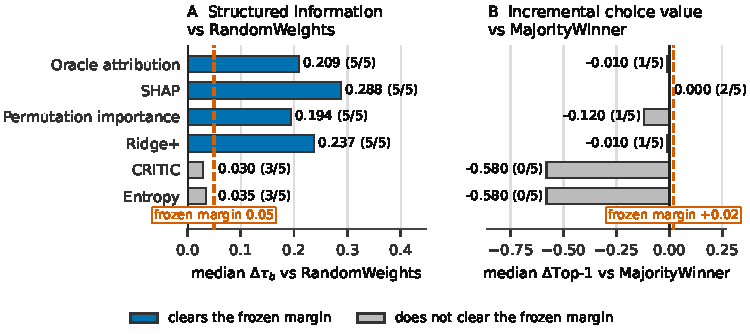
\includegraphics[width=\linewidth]{decision_value_figure}
\caption{Information learned is not decision value added. Left: every structured
method except \CRITIC{} and entropy clears the frozen $0.05$ Kendall margin against
RandomWeights. Right: no method reaches the frozen $+0.02$ Top-1 margin against the
constant MajorityWinner reference, and SHAP's advantage there is exactly zero. Both
panels are drawn directly from the frozen Pilot-B result on a common untruncated
scale.}
\label{fig:contrast}
\end{figure}

The exact oracle-attribution reference failed the same gate, so the stop cannot be
attributed to \XGB{} fitting error or TreeSHAP approximation alone.

\subsection{Post-Closure Descriptive Selection Maps}
\label{sec:selectionmaps}

The Pilot-B artefact retained aggregate metrics but not method-level context
selections. After permanent closure, a separate protocol was frozen before any
selection was reconstructed. It reused the archived fixed weights and TEST identities,
generated no target, fitted or queried no model, re-estimated no weight, and could not
alter the gate; an independent audit verified all $5\times7\times200=7000$ selections.
This is a post-closure descriptive diagnostic and has no confirmatory role.

Equal-weight \MOORA{} selected a single alternative in every context of every world and
matched MajorityWinner exactly in four of five worlds. Structured-method constancy was
heterogeneous, from zero worlds for PI to three for entropy
(Table~\ref{tab:selectionmaps}). The simple hypothesis that every fixed-weight \MOORA{}
vector must be context invariant is therefore not supported for the seven observed
vectors. World 21003 also shows why Top-1 and full-ranking fidelity must be reported
separately: Equal, \CRITIC{} and entropy all selected $A_6$ in all $200$ contexts,
giving identical Top-1 accuracy $0.190$ and mean regret $0.316758$, while their mean
$\tau_b$ values still differed ($0.5493$, $0.5427$, $0.5113$) because the lower ranks
differed. These observations suggest locally coarse decision regions for particular
fixed vectors. They do not characterize unobserved weight space, do not establish a
causal mechanism for the Pilot-B stop, and do not change its outcome.

\begin{table}[t]
\centering
\caption{Post-closure descriptive diagnostic over the seven observed fixed vectors.
Counts give worlds with a single selected alternative, and worlds with exact
context-level agreement with MajorityWinner. Descriptive only; non-confirmatory.}
\label{tab:selectionmaps}
\small
\begin{tabular}{@{}l@{\hspace{2em}}c@{\hspace{2em}}c@{}}
\toprule
Method & Constant-selection worlds & All-context MW-match worlds\\
\midrule
Oracle attribution & 1/5 & 1/5\\
SHAP & 2/5 & 2/5\\
Permutation importance & 0/5 & 0/5\\
Ridge+ & 1/5 & 1/5\\
CRITIC & 2/5 & 1/5\\
Entropy & 3/5 & 2/5\\
Equal & 5/5 & 4/5\\
\bottomrule
\end{tabular}
\end{table}

% ============================================================
\section{Discussion}
\label{sec:discussion}
% ============================================================

\subsection{What the Study Establishes}
\label{sec:establishes}

RQ1 and RQ2 are addressed by the prospectively structured benchmark-development and
Pilot-B evidence. The separately frozen post-closure diagnostic addresses DQ1
descriptively and has no confirmatory role.

For RQ1, an algebraic and numerical audit showed that contextual variation can vanish
entirely under the normalization used by the decision operator, and that a diagnostic
must be applied at that point to detect it. For RQ2, correcting exact separability
produced multiple oracle orderings and winners in every world, but it did not establish
sufficient incremental decision value: no structured global-weight pipeline escaped
MajorityWinner under the frozen cross-world rule.

The clearest reading is not that SHAP failed. Its separation from RandomWeights shows
that its weights carried reproducible ranking information, and that entire median
advantage then disappeared against a single constant choice: at this reference
condition the bottleneck lay in converting one global weight vector into
context-specific decision value through \MOORA{}. Because closed-form oracle
attribution reached the same outcome, an explanation resting solely on imperfect
learned attribution is ruled out. No single causal mechanism is isolated, however:
generator geometry, global compression, reference construction and \MOORA{} geometry
remain coupled in the executed design.

For applied OR and transport research the lesson is compact. A complex data-driven
pipeline should be compared not only against random or uniform parameters but also
against a meaningful simple decision policy: beating random weights shows that
information was learned, not that it usefully changes the operational choice.

\subsection{Interpretation Boundary and Limitations}
\label{sec:limits}

The central boundary statement is this. \emph{Pilot-B failure denotes failure of the
prespecified adequacy requirement for the intended global-weight--\MOORA{} comparison;
it does not imply that the generator contains no discriminative decision information.}
Four independent observations support the distinction: RandomWeights decisions were not
invariant; four structured methods separated from RandomWeights; SHAP held a large and
consistent Kendall advantage; and the observed fixed vectors displayed heterogeneous
selection constancy rather than uniform collapse. Equally, the result does not show
that SHAP universally fails, that global weights never matter, that \MOORA{} is
generally inadequate, that the D29 kernel is defective, that one ITS alternative is
best, or that MajorityWinner should be deployed.

Ten limitations bound the claim.

\begin{enumerate}
\itemsep1pt
\item Pilot B uses only five worlds, so cross-world inferential precision is low.
\item Those five are reused development worlds, not fresh ones.
\item Only one reference condition was evaluated, $(N,c,\rho,\lambda)=(250,0.30,0.4,0.5)$.
\item \emph{Prospective freezing prevents post-result modification of the gate, but it
does not make the five reused development worlds independent validation data.} The
result is a protocol-level adequacy screen; no population-level inference about method
performance is claimed.
\item MajorityWinner headroom varies strongly across worlds, from a modal share of
$0.519$ to $0.983$, so the difficulty of the comparison is itself heterogeneous.
\item MajorityWinner is Top-1-derived, not regret-optimal. The regret arm uses the same
prospectively frozen Top-1-derived constant reference rather than a separately
optimized regret-minimizing constant policy. A future benchmark could prospectively
define metric-matched constant references.
\item The generator, oracle and capability mask are synthetic assumptions, not
empirical transport effects, causal truth, stakeholder preferences or social welfare.
\item Every global-weight method intentionally compresses context-specific information,
and the methods differ in semantics: oracle attribution and SHAP target one
interventional functional; Ridge+ and PI use supervised association; \CRITIC{} and
entropy summarize pooled decision-matrix properties. PI can additionally extrapolate
when dependence is broken \cite{hooker2021permutation}.
\item The post-closure diagnostic adds no independent worlds. A paired context
bootstrap was prospectively excluded from that layer and was not executed; any
resampling study would require its own protocol and could not reopen the gate.
\item The paper makes no empirical ITS deployment recommendation.
\end{enumerate}

The negative result stays scientifically useful because it was not tuned away. The
generator correction, the gate thresholds, the evaluator and the seed firewall all
preceded the authorized result. Once the modal-winner stop fired, the 30-world primary
factorial and the reserve worlds remained barred. Any future design must begin as a
separately versioned study that discloses this closed result rather than retroactively
amending it.

% ============================================================
\section{Conclusion}
\label{sec:conclusion}
% ============================================================

This study asked whether a synthetic ITS benchmark could support a global XAI--MCDM
method comparison, and it asked before running the comparison at scale. Structural
auditing found and corrected a normalization-induced collapse in the original
generator, but that correction, while necessary, did not by itself establish downstream
decision discrimination. At the frozen development reference, four structured
methods---SHAP among them---cleared the RandomWeights adequacy criterion, yet none
cleared the MajorityWinner criterion, and closed-form oracle attribution failed the
same gate.

The defensible conclusion is narrow and actionable: at this reference condition the
evaluated global-weight-compression--\MOORA{} pipelines did not establish enough
incremental decision value to justify the protected primary factorial, and the gate
therefore performed its intended function. More broadly, synthetic XAI--MCDM studies
should validate not only prediction and attribution, but also whether the benchmark can
discriminate decisions beyond meaningful simple references. In XAI-assisted decision
support, recovering structured importance is not enough; the recovered information must
demonstrably change decisions in a useful way.

% ============================================================
\section*{Code and Data Availability}

The reproducibility package contains the synthetic benchmark generator, the frozen
configuration and protocol files, the deterministic seed definitions, the archived
development-audit and Pilot-B result artefacts, the frozen global-weight vectors, the
post-closure selection-map outputs, the independent audit and evaluator scripts, the
software-environment specification, content-integrity manifests, and the read-only
scripts that regenerate every table and figure reported here. Raw benchmark worlds are
regenerated deterministically from the frozen seeds and configurations rather than
stored as large duplicated datasets. Primary and reserve worlds were never accessed and
no primary result exists.
\ifanon
During double-blind review, identifying repository metadata is withheld; an anonymous
archive can be supplied to editors and reviewers on request. The complete
version-controlled repository and its immutable provenance record will be released
publicly after review.
\else
The complete version-controlled repository and its immutable provenance record are
released with the public reproducibility package.
\fi

\ifanon
\else
\section*{CRediT Authorship Contribution Statement}

\textbf{Mohamed Yassine Neifar:} Conceptualization, Methodology, Software, Validation,
Formal analysis, Investigation, Data curation, Visualization, Writing -- original
draft, Writing -- review and editing.
\textbf{Nadir Farhi:} Conceptualization, Methodology, Validation, Supervision,
Writing -- review and editing.
\textbf{Ahmed Frikha:} Supervision, Writing -- review and editing.
\fi

\section*{Funding}

This research did not receive any specific grant from funding agencies in the public,
commercial, or not-for-profit sectors.

\section*{Declaration of Competing Interest}

The authors declare that they have no known competing financial interests or personal
relationships that could have appeared to influence the work reported in this paper.

\section*{Declaration of Generative AI and AI-Assisted Technologies}

Generative AI tools were used for language editing, manuscript organization,
consistency checking and LaTeX assistance. All scientific design decisions, code
executions, numerical results, interpretations and citations were independently checked
by the authors, who take full responsibility for the manuscript.

\ifanon
\else
\section*{Acknowledgements}

The authors acknowledge the academic guidance and scientific support provided within
the doctoral research collaboration between the University of Sfax and Universit\'e
Gustave Eiffel.
\fi

% ============================================================
\begin{thebibliography}{99}

\bibitem{keeney1976decisions}
Keeney, R.L., Raiffa, H.:
Decisions with Multiple Objectives: Preferences and Value Tradeoffs.
Wiley, New York (1976).

\bibitem{roy1996importance}
Roy, B., Mousseau, V.:
A theoretical framework for analysing the notion of relative importance of criteria.
Journal of Multi-Criteria Decision Analysis \textbf{5}(2), 145--159 (1996).
\url{https://doi.org/10.1002/(SICI)1099-1360(199606)5:2<145::AID-MCDA99>3.0.CO;2-5}

\bibitem{choo1999weights}
Choo, E.U., Schoner, B., Wedley, W.C.:
Interpretation of criteria weights in multicriteria decision making.
Computers \& Industrial Engineering \textbf{37}(3), 527--541 (1999).
\url{https://doi.org/10.1016/S0360-8352(00)00019-X}

\bibitem{mukhametzyanov2021objective}
Mukhametzyanov, I.:
Specific character of objective methods for determining weights of criteria in MCDM
problems: Entropy, CRITIC and SD.
Decision Making: Applications in Management and Engineering \textbf{4}(2), 76--105
(2021).
\url{https://doi.org/10.31181/dmame210402076i}

\bibitem{chen2016xgboost}
Chen, T., Guestrin, C.:
XGBoost: A scalable tree boosting system.
In: Proceedings of the 22nd ACM SIGKDD International Conference on Knowledge Discovery
and Data Mining, pp. 785--794 (2016).
\url{https://doi.org/10.1145/2939672.2939785}

\bibitem{lundberg2017shap}
Lundberg, S.M., Lee, S.-I.:
A unified approach to interpreting model predictions.
In: Advances in Neural Information Processing Systems, vol. 30 (2017).

\bibitem{lundberg2020trees}
Lundberg, S.M., Erion, G., Chen, H., et al.:
From local explanations to global understanding with explainable AI for trees.
Nature Machine Intelligence \textbf{2}, 56--67 (2020).
\url{https://doi.org/10.1038/s42256-019-0138-9}

\bibitem{sundararajan2020many}
Sundararajan, M., Najmi, A.:
The many Shapley values for model explanation.
In: Proceedings of the 37th International Conference on Machine Learning,
PMLR \textbf{119}, 9269--9278 (2020).

\bibitem{kumar2020shapleyproblems}
Kumar, I.E., Venkatasubramanian, S., Scheidegger, C., Friedler, S.:
Problems with Shapley-value-based explanations as feature importance measures.
In: Proceedings of the 37th International Conference on Machine Learning,
PMLR \textbf{119}, 5491--5500 (2020).

\bibitem{janzing2020causal}
Janzing, D., Minorics, L., Bl{\"o}baum, P.:
Feature relevance quantification in explainable AI: A causal problem.
In: Proceedings of the 23rd International Conference on Artificial Intelligence and
Statistics, PMLR \textbf{108}, 2907--2916 (2020).

\bibitem{hooker2021permutation}
Hooker, G., Mentch, L., Zhou, S.:
Unrestricted permutation forces extrapolation: Variable importance requires at least
one more model, or there is no free variable importance.
Statistics and Computing \textbf{31}, 82 (2021).
\url{https://doi.org/10.1007/s11222-021-10057-z}

\bibitem{liu2021xaibench}
Liu, Y., Khandagale, S., White, C., Neiswanger, W.:
Synthetic benchmarks for scientific research in explainable machine learning.
Proceedings of the Neural Information Processing Systems Track on Datasets and
Benchmarks \textbf{1} (2021).

\bibitem{agarwal2022openxai}
Agarwal, C., Krishna, S., Saxena, E., Pawelczyk, M., Johnson, N., Puri, I., Zitnik, M.,
Lakkaraju, H.:
OpenXAI: Towards a transparent evaluation of model explanations.
In: Advances in Neural Information Processing Systems, vol. 35, Datasets and Benchmarks
Track (2022).

\bibitem{ciano2025xaimcdm}
Ciano, T., Ferrara, M.:
Explainable multi-criteria decision making for tourism economics: Integrating XAI with
MCDM for a robust accommodation performance assessment.
Decisions in Economics and Finance (2025).
\url{https://doi.org/10.1007/s10203-025-00553-6}

\bibitem{demir2025shapmultimoora}
Demir, A.S., Da{\u g}deviren, U., Kurnaz, T.F., Erden, C., K{\"o}k{\c c}am, A.H.:
An integrated SHAP-MCDM approach for slope stability prediction based on machine
learning algorithms.
Natural Hazards \textbf{121}(18), 21811--21836 (2025).
\url{https://doi.org/10.1007/s11069-025-07665-7}

\bibitem{zakeri2024mlmcdm}
Zakeri, S., Konstantas, D., Sorooshian, S., Chatterjee, P.:
A novel ML-MCDM-based decision support system for evaluating autonomous vehicle
integration scenarios in Geneva's public transportation.
Artificial Intelligence Review \textbf{57}, 310 (2024).
\url{https://doi.org/10.1007/s10462-024-10917-w}

\bibitem{diakoulaki1995critic}
Diakoulaki, D., Mavrotas, G., Papayannakis, L.:
Determining objective weights in multiple criteria problems: The CRITIC method.
Computers \& Operations Research \textbf{22}(7), 763--770 (1995).
\url{https://doi.org/10.1016/0305-0548(94)00059-H}

\bibitem{shannon1948}
Shannon, C.E.:
A mathematical theory of communication.
Bell System Technical Journal \textbf{27}, 379--423, 623--656 (1948).

\bibitem{brauers2006moora}
Brauers, W.K.M., Zavadskas, E.K.:
The MOORA method and its application to privatization in a transition economy.
Control and Cybernetics \textbf{35}(2), 445--469 (2006).

\bibitem{fhwa2016corridors}
Federal Highway Administration:
Planning for Transportation Systems Management and Operations Within Corridors: A Desk
Reference, FHWA-HOP-16-037 (2016).
\url{https://ops.fhwa.dot.gov/Publications/fhwahop16037/}

\bibitem{fhwa2017atm}
Kuhn, B., Balke, K., Wood, N.:
Active Traffic Management (ATM) Implementation and Operations Guide.
FHWA-HOP-17-056, Federal Highway Administration (2017).
\url{https://ops.fhwa.dot.gov/publications/fhwahop17056/}

\bibitem{usdotv2x}
U.S. Department of Transportation, ITS Joint Program Office:
V2X Applications and Use Cases.
\url{https://its.dot.gov/research-areas/V2X-Deployment/overview/v2x-applications/}
(accessed 13 August 2026).

\bibitem{morris2019simulation}
Morris, T.P., White, I.R., Crowther, M.J.:
Using simulation studies to evaluate statistical methods.
Statistics in Medicine \textbf{38}(11), 2074--2102 (2019).
\url{https://doi.org/10.1002/sim.8086}

\bibitem{niessl2022overoptimism}
Nie{\ss}l, C., Herrmann, M., Wiedemann, C., Casalicchio, G., Boulesteix, A.-L.:
Over-optimism in benchmark studies and the multiplicity of design and analysis options
when interpreting their results.
WIREs Data Mining and Knowledge Discovery \textbf{12}(2), e1441 (2022).
\url{https://doi.org/10.1002/widm.1441}

\end{thebibliography}

\end{document}
